%\documentclass[ms,electronic,twosidetoc,letterpaper,chaptercenter,parttop,lof,lot]{byumsphd}
\documentclass[ms,electronic,oneside,letterpaper,chaptercenter,parttop,lof,lot]{byumsphd}
% Author: Chris Monson
%
% This document is in the public domain
%
% Options for this class include the following (* indicates default):
%
%   phd (*) -- produce a dissertation
%   ms -- produce a thesis
%
%   electronic -- default official university option, overrides the following:
%                 - equalmargins
%
%   hardcopy -- overrides the following:
%                 - no equalmargins
%                 - twoside
%
%   letterpaper -- ignored, but helpful for the Makefile that I use
%
%   10pt -- 10 point font size
%   11pt -- 11 point font size
%   12pt (*) -- 12 point font size
%
%   lof -- produce a list of figures in the preamble (off)
%   lot -- produce a list of tables in the preamble (off)
%   lol -- produce a list of listings in the preamble (off)
%
%   layout -- show layout lines on the pages, helps with overfull boxes (off)
%   grid -- show a half-inch grid on every page, helps with printing (off)
%   separator -- print an extra instruction page between preamble and body (off)
%
%   twoside (*) -- two-sided output (margins alternate for odd and even pages,
%     blank pages inserted to ensure that chapters begin on the right side of a
%     bound copy, etc.)
%   oneside -- one-sided output (margins are the same on all pages)
%   equalmargins -- make all margins equal - ugly for binding, but compliant
%
%   twosidetoc - start two-sided margins at the TOC instead of the body.  This
%     is sometimes (oddly) required, but be aware that it will make the page
%     numbering seem screwy, e.g., the first four full sheets of paper will
%     have number i-iv (not shown, though), and the next sheets will each have
%     two numbers, one for each side.  I suspect that most people don't look at
%     the roman numerals anyway, but it is a weird requirement.
%
%   openright (*) -- force new chapters to start on an odd page
%   openany -- don't use this, it's ugly
%
%   prettyheadings -- make the section/chapter headings look nice
%   compliantheadings (*) -- make them look ugly, but compliant with standards
%
%   chaptercenter -- center the chapter headings horizontally
%   chapterleft (*) -- place chapter headings on the left
%
%   partmiddle -- Part headers are centered vertically, no other text on page
%   parttop (*) -- Part headers at top of page, other text expected
%
%   duplexprinter -- Ensures that the two-sided portion starts on the right
%     side when printing.  This is not for use in submission, since the best
%     thing to do there is to print everything out one-sided, then take it down
%     to the copy store to have them do the rest.  It does help to save trees
%     when you are printing out copies just to look at them and fiddle with
%     things.
%
%
% EXAMPLES:
%
% The rest is up to you.  To fiddle with margins, use the \settextwidth and
% \setbindingoffset macros, described below.  I suggest that you
% \settextwidth{6.0in} for better-looking output (otherwise you'll get 3/4-inch
% margins after binding, which is sort of weird).  This will depend on the
% opinions of the various dean/coordinator folks, though, so be sure to ask
% them before embarking on a major formatting task.

% The following command fixes my particular printer, which starts 0.03 inches
% too low, shifting the whole page down by that amount.  This shifts the
% document content up so that it comes out right when printed.
%
% Discovering this sort of behavior is best done by specifying the ``grid''
% option in the class parameters above.  It prints a 1/2 inch grid on every
% page.  You can then use a ruler to determine exactly what the printer is
% doing.
%
% Uncomment to shift content up (accounting for printer problems)
%\setlength{\voffset}{-.03in}

% Here we set things up for invisible hyperlinks in the document.  This makes
% the electronic version clickable without changing the way that the document
% prints.  It's useful, but optional.
%
% NOTE: "driverfallback=ps2pdf" chooses ps2pdf in the case of LaTeX and pdftex
% in the case of pdflatex. If you use my LaTeX makefile (at
% http://latex-makefile.googlecode.com/) then pdftex is the default There are
% many other benefits to using the makefile, too.  This option is not always
% available, so use with care.
\usepackage[
    bookmarks=true,
    bookmarksnumbered=true,
    breaklinks=false,
    raiselinks=true,
    pdfborder={0 0 0},
    colorlinks=false,
    plainpages=false,
    ]{hyperref}

%\usepackage[pass]{geometry}
\usepackage{verbatim}
\usepackage{url}
\usepackage{color}
\usepackage{multicol}
\usepackage{paralist}
\usepackage{comment}
\usepackage{graphicx}
\usepackage{amsmath, listings, amsthm, amssymb, proof, xspace, stmaryrd, times}
\usepackage{subfigure}
%\usepackage{cite}
\usepackage[nounderscore]{syntax}
\usepackage{newfloat}
\usepackage{esvect}
\usepackage{semantic}
\usepackage{mathpartir}
\usepackage{pdflscape}

\DeclareFloatingEnvironment[
  % the file extension for the file used to create the list:
  fileext   = logr,% don't use log here!
  % the heading for the list:
  listname  = {List of Grammars},
  % the name used in captions:
  name      = Grammar,
  % the default floating parameters if the environment is used
  % without optional argument:
  placement = htp
]{Grammar}

\newcommand{\figref}[1]{Figure~\ref{#1}}
\newcommand{\lemmaref}[1]{Lemma~\ref{#1}}
\newcommand{\tableref}[1]{Table~\ref{#1}}
\newcommand{\secref}[1]{Section~\ref{#1}}
\newcommand{\lineref}[1]{Line~\ref{#1}}
\newcommand{\corref}[1]{Corollary~\ref{#1}}
\newcommand{\thmref}[1]{Theorem~\ref{#1}}
\newcommand{\algoref}[1]{Algorithm~\ref{#1}}

\newcommand{\setof}[1]{\ensuremath{\left \{ #1 \right \}}}
\newcommand{\tuple}[1]{\ensuremath{\langle #1 \rangle }}

\newcommand{\mystar}{{\fontfamily{lmr}\selectfont$\star$}}

\definecolor{dkgreen}{rgb}{0,0.6,0}
\definecolor{gray}{rgb}{0.5,0.5,0.5}
\definecolor{mauve}{rgb}{0.58,0,0.82}


\lstset{frame=tb,
  language=Java,
  aboveskip=3mm,
  belowskip=3mm,
  showstringspaces=false,
  columns=flexible,
  %basicstyle={\small\ttfamily},
  numbers=none,
  numberstyle=\tiny\color{gray},
  %keywordstyle=\color{blue},
  commentstyle=\color{dkgreen},
  stringstyle=\color{mauve},
  breaklines=true,
  breakatwhitespace=true,
  tabsize=3,
  morekeywords={proc, post, await, ewait, var, skip, assume, call, return}
}

\newtheorem{definition}{Definition}
\newtheorem{theorem}{Theorem}
\newtheorem{lemma}{Lemma}
\newtheorem{corollary}{Corollary}

\usepackage{algorithm, algpseudocode}

%%------------------------------------------------------------------------
%% DEFINITION HELPERS
%%------------------------------------------------------------------------

\newcommand{\alt}{~~|~~}
\iffalse
\newcommand{\comp}[1]{\llbracket #1 \rrbracket}
\fi

\newcommand{\inlinexp}[1]{
{\footnotesize
 \[\begin{array}{l}
 #1
 \end{array}\]}}

\newcommand{\inlinexpa}[2]{
{\footnotesize
 \[\begin{array}{#1}
 #2
 \end{array}\]}}

\newcommand{\infr} [3] [] {\infer[\textsc{#1}]{#3}{#2}}
\newcommand{\iand}        {\qquad}

\newcommand{\Ctxt}       {\mathcal{E}}
\newcommand{\InCtxt} [1] {\Ctxt[#1]}

%%------------------------------------------------------------------------
%% REDUCTION RELATION MACROS
%%------------------------------------------------------------------------

\newcommand{\subst} [3]    {#3 [#2 / #1]}
\newcommand{\dstep} [2]    {#1 ~\Downarrow~ #2}

\newcommand{\ssosredex}        {\rightarrow}
\newcommand{\ctxtreduce}       {\mapsto}
\newcommand{\sstep}     [3] [] {#2 &\ssosredex&  #3 &\textsc{#1}}
\newcommand{\ctxtstep}  [3] [] {#2 &\ctxtreduce& #3 &\textsc{#1}}

%%------------------------------------------------------------------------
%% TYPE DEFINITION MACROS
%%------------------------------------------------------------------------

\newcommand{\funct} [2] {#1\nobreak\rightarrow\nobreak#2}
\newcommand{\boolt}     {\mathtt{bool}}

\newcommand{\typeEnv}         {\Gamma}
\newcommand{\entails}         {\vdash}
\newcommand{\judgment}   [3] {#1 \entails #2 : #3}
\newcommand{\envent}      [2] {\judgment{\typeEnv}{#1}{#2}}
\newcommand{\extenvent}   [4] {\judgment{\typeEnv, #1 : #2}{#3}{#4}}
\newcommand{\envlookup}   [3] {\infr{#1(#2) = #3}{\judgment{#1}{#2}{#3}}}

%%------------------------------------------------------------------------
%% EXPRESSION MACROS
%%------------------------------------------------------------------------

%% lambda
\newcommand{\lamdefe}  [2] {\lambda #1.~#2}
\newcommand{\lamdefea} [2] {\begin{array}{l}\lambda#1.\\\hspace*{.5em}#2\\\end{array}}

%% let
\newcommand{\letdefe}    [3] {\letbind{#1}{#2}~\letin{#3}}
\newcommand{\letdefarre} [3] {\begin{array}{l}\letbind{#1}{#2}\\\letin{#3})\\\end{array}}

\newcommand{\letbind}  [2] {\mathsf{let}~\lbind{#1}{#2}}
\newcommand{\letbindp} [2] {\mathsf{let}~(\lbind{#1}{#2})}
\newcommand{\lbind}    [2] {#1=#2}
\newcommand{\letin}    [1] {\mathsf{in}~#1}

%% if
\newcommand{\ife}      [3] {\ifline{#1}~\thenline{#2}~\elseline{#3}}
\newcommand{\ifea}     [3] {\begin{array}{l}\ifline{#1}\\\thenline{#2}\\\elseline{#3}\end{array}}

\newcommand{\ifop}         {\mathsf{if}}
\newcommand{\ifline}   [1] {\ifop~ #1}
\newcommand{\thenline} [1] {\mathsf{then}~#1}
\newcommand{\elseline} [1] {\mathsf{else}~#1}

%% opers
\newcommand{\binopdef}     {\mathit{binop}}
\newcommand{\unopdef}      {\mathit{unop}}
\newcommand{\binope}   [2] {\binopdef~#1~#2}
\newcommand{\unope}    [1] {\unopdef~#1}

\newcommand{\andop}        {\mathsf{and}}
\newcommand{\orop}         {\mathsf{or}}
\newcommand{\notop}        {\mathsf{not}}
\newcommand{\ande}     [2] {\mathsf{and}~#1~#2}
\newcommand{\ore}      [2] {\mathsf{or}~#1~#2}
%\newcommand{\note}     [1] {\mathsf{not}~#1}

%% values
\newcommand{\falsev}     {\mathsf{false}}
\newcommand{\truev}      {\mathsf{true}}


% These packages allow the bibliography to be sorted alphabetically and allow references to more than one paper to be sorted and compressed (i.e. instead of [5,2,4,6] you get [2,4-6])
\usepackage[numbers,sort&compress]{natbib}
\usepackage{hypernat}

% Because I use these things in more than one place, I created new commands for
% them.  I did not use \providecommand because I absolutely want LaTeX to error
% out if these already exist.
\newcommand{\Title}{Verification of Task Parallel Programs using Predictive Analysis}
\newcommand{\Author}{Radha Nakade}
\newcommand{\GraduationMonth}{August}
\newcommand{\GraduationYear}{2016}

% Set up the internal PDF information so that it becomes part of the document
% metadata.  The pdfinfo command will display this.
\hypersetup{%
    pdftitle=\Title,%
    pdfauthor=\Author,%
    pdfsubject={MS Thesis, BYU CS Department: %
                Degree Granted \GraduationMonth~\GraduationYear, Document Created \today},%
    pdfkeywords={BYU, thesis},%
}

% Rewrite the itemize, description, and enumerate environments to have more
% reasonable spacing:
\newcommand{\ItemSep}{\itemsep 0pt}
\let\oldenum=\enumerate
\renewcommand{\enumerate}{\oldenum \ItemSep}
\let\olditem=\itemize
\renewcommand{\itemize}{\olditem \ItemSep}
\let\olddesc=\description
\renewcommand{\description}{\olddesc \ItemSep}

% Important settings for the byumsphd class.
\title{\Title}
\author{\Author}

\committeechair{Eric Mercer}
\committeemembera{Quinn Snell}
\committeememberb{Parris Egbert}

%\monthgraduated{\GraduationMonth}
%\yeargraduated{\GraduationYear}
\yearcopyrighted{\GraduationYear}

\documentabstract{
Task parallel programming languages provide a way for creating asynchronous tasks that can run concurrently. The advantage of using task parallelism is that the programmer can write code that is independent of the underlying hardware. The runtime determines the number of processor cores that are available and the most efficient way to execute the tasks. When two or more concurrently executing tasks access a shared memory location and if at least one of the accesses is for writing, data race is observed in the program. Data races can introduce non-determinism in the program output making it important to have data race detection tools. To detect data races in task parallel programs, a new sound and complete technique based on computation graphs is presented in this work. The data race detection algorithm runs in $\mathcal{O}$(N$^2$) time where N is number of nodes in the graph. A computation graph is a directed acyclic graph that represents the execution of the program. For detecting data races, the computation graph stores shared heap locations accessed by the tasks. An algorithm for creating computation graphs augmented with memory locations accessed by the tasks is also described here. This algorithm runs in $\mathcal{O}$(N) time where N is the number of operations performed in the tasks. A scheduling algorithm that creates all possible computation graph structures for programs containing critical sections is also presented here. This work also presents an implementation of this technique for the Java implementation of the Habanero programming model. The results of this data race detector are compared to Java Pathfinder's precise race detector extension and permission regions based race detector extension. The results show a significant reduction in the time required for data race detection using this technique.
}

\documentkeywords{%
    verification, task parallel programming, data race detection
}

\acknowledgments{%
I would like to thank my advisor, Dr. Eric Mercer for his constant motivation and his patience. This work wouldn't have been possible without his help. I would also like to thank Dr. Jay McCarthy and my committee members for their feedback in the project.

I am grateful to my family for their love and support. And finally, I want to thank my wonderful husband, Atul for his support, love and encouragement. 
}

\department{Computer~Science}
\graduatecoordinator{Quinn Snell}
\collegedean{Thomas~W.~Sederberg}
\collegedeantitle{Associate~Dean}

% Customize the name of the Table of Contents section.
\renewcommand\contentsname{Table of Contents}

% Remove all widows an orphans.  This is not normally recommended, but in a
% paper dissertation there is no reasonable way around it; you can't exactly
% rewrite already-published content to fix the problem.
\clubpenalty 10000
\widowpenalty 10000

% Allow pages to have extra blank space at the bottom in order to accommodate
% removal of widows and orphans.
\raggedbottom

% Produce nicely formatted paragraphs. There is nothing additional to do.  In
% case you get some problems, surround your text with
% \begin{sloppy} ... \end{sloppy}. If that does not work, try
% \microtypesetup{protrusion=false} ... \microtypesetup{protrusion=true}
\usepackage{microtype}

\begin{document}

% Produce the preamble
\microtypesetup{protrusion=false}
\maketitle
\microtypesetup{protrusion=true}

\chapter{Introduction}
\section{Introduction}
Despite the explosion in multi-core hardware for general purpose
computing, writing programs to take advantage of the available
processing power is a task reserved for expert
developers. Parallel programming models are nuanced with non-trivial 
language semantics, and the first programs from the uninitiated have
more in common with sequential execution than parallel performance due
to excessive synchronization, or worse, those programs are
fraught with concurrency errors due to an absence of needed
synchronization. Parallel semantics is not the normal mental model for
most programmers, and as a result, parallelism is employed little,
deployed incorrectly, or exclusively reserved for the expert users
which are not found in abundance.

The Habanero extreme scale software research project intends to bring
multi-core programming to the masses by providing languages,
compilers, run-time systems, and tools to support programmers that are
not experts in concurrency. Habanero itself is a task-parallel
programming model built around lightweight asynchronous tasks and data
transfers. As such, rather than manipulating processes, threads, and
synchronization for concurrent execution, the programmer identifies
sections of the program that can run concurrently as tasks using
simple annotations in the sequential code. An implementation of
Habanero would then shoulder the complexity of the parallel execution
and absolve the programmer of that responsibility. The
programmer now focuses on the high-level task constructs while an
implementation worries about how to correctly implement and
synchronize those constructs.

Aside from the simplified task-parallel programming model, Habanero
gives some limited correctness guarantees. It defines safe subsets of
the language that preserve correctness in regards to concurrent
interactions. For example, programs that only create tasks and join
on their termination are free of deadlock, support serialization (i.e.,
removing all the annotations yields a sequential program that gives
the same computation), and in the absence of data-race (i.e.,
conflicting concurrent accesses to shared memory), those same programs
are deterministic. In a safe subset, a programmer does not need to
worry about concurrent interactions between tasks beyond data-race.

Habanero Java (\hj) is the most widely deployed implementation of the
Habanero model, and it has been adopted as a pedagogical language for
teaching concurrency \cite{Cave:2011:HNA:2093157.2093165}; however,
there is a gap between the theory of the language with its safe subsets
and the implementation in regards to test and validation.  When operating
within a safe subset of the language or outside for
performance, there is no easy way to determine when and if a program
is free of data-race---a necessary condition for determinism. Even
debugging computation is non-trivial as the \hj\ implementation is
complex, so a user has no obvious method to track a task, let alone
control its execution, using a conventional debugger. As a result,
inefficient code inspection, run-time failures, and
\emph{printf}-debugging are the primary techniques for test and validation.

This paper presents research to address debugging, test, and
validation for task parallel programming models such as Habanero. The
first contribution is a new implementation of Habanero for Java in the
form of a library (\hjv). The implementation trades performance for
simplicity and correctness. It does this by using Java threads for
each task, and using global locks with conditions for features of
Habanero that require mutual exclusion and complex synchronization. As
such, it is well suited for test and validation since a conventional
debugger is able to inspect and control the execution of tasks (e.g.,
Java threads). Additionally, weighing in with only 32
classes and around 1,300 lines of code, the library is an
order of magnitude less complex than even the most simple
implementations in the \hj\ distribution. Careful manual inspection of
the code base, which is conveniently small, with extensive testing and
verification, reasonably ensure a high degree of confidence in its correctness and supports the
claim that \hjv\ preserves all behaviors allowed by the Habanero
semantics. That said, finding deadlock and data-race in an input
program is still a difficult challenge as is enumerating behaviors for test in non-deterministic programs.

The \hjv\ library enables model checking for \hj\ programs. Model
checking exhaustively enumerates program behavior, and in the case of
task-parallel programming models, it reasons over task schedules to
prove the absence of errors. The Java Pathfinder model checker (\jpf)
is able to directly verify freedom from deadlock and data-race in
\hj\ programs using \hjv\ as the Habanero implementation because \hjv\ employs a one-to-one
mapping between tasks and threads. The verification leverages the
native support for threads and locks in \jpf\ to automatically explore all possible
ways to schedule concurrent tasks. Such an approach is not possible
using the other Habanero implementations in the \hj\ distribution
because \jpf\ does not know where to schedule. The model checking is effective for verifying the
\hjv\ implementation beyond manual inspection and proving small
programs correct, but it does not scale to larger programs.

The second contribution to debugging, test, and validation is an
implementation in \jpf\ of a sound algorithm for the validation of
task-parallel programming models such as Habanero that is able to
detect programs that are free of deadlock and data-race (\jpfhj). It also enumerates all outcomes that arise from non-determinism in sequencing isolated atomic blocks. The
algorithm still employs model checking with the \hjv\ library as
before; however, to scale to larger input programs, the algorithm uses
permission regions to annotate atomic blocks of read/write operations
on shared memory. These atomic blocks effectively reduce the number of
schedules that must be considered to prove a program correct.

Permission regions are program annotations that announce how a task
interacts with shared memory (i.e., reading or writing), and over what
region of code that interaction takes place
\cite{Westbrook:2011:PRR:2341616.2341627,
  Westbrook:2012:PPR:2367163.2367201}. During execution, auxiliary
data structures track access on those memory regions and signal an
error on any conflicting access. Permission regions have been shown
effective in dynamically detecting data-race at run-time.

\jpfhj\ includes an implementation of permission regions and a
specialized scheduling algorithm to reduce the number of explored
schedules needed to show a program free of deadlock and data-race. The
new algorithm only preempts at the entrance to permission regions and isolated atomic blocks to
schedule threads.  As stated previously, the new algorithm is sound,
meaning that it may reject programs that are actually correct if the
permission regions are too big, but effective at controlling state explosion. The
algorithm does report a witness to any discovered deadlock or
data-race violation which can be used to validate the error with the
debugger. If the error is a false report due to the size of the
regions, then the witness provides insight on how to reduce the size of
the permission regions. This new algorithm together with the
simplified run-time provide needed support for debug, test, and
validation of task parallel programs.

The principle contributions described in this paper are summarized as
\begin{compactitem}
\item \hjv: a verification specific implementation of Habanero for Java as a Java library that is extensively tested through model checking with \jpf\ and is amenable to conventional debugging;
\item \jpfhj: an implementation of permission regions in the \jpf\ model checker with a sound algorithm that only schedules on permission regions and isolated atomic blocks to prove a program free of deadlock and data-race; and 
\item an empirical study showing the impact of permission regions on the complexity of model checking over a set of benchmarks.
\end{compactitem}
The \hjv\ library and \jpfhj\ specialization are available for
download at: \url{http://javapathfinder.org/jpf-hj/}.


\chapter{Data Race Detection}
A computation graph for a task parallel program is a directed acyclic graph that represents the execution of the program. The graph consists of nodes that denote the various parallel operations. The nodes also store references to the memory locations accessed by the tasks.

\begin{definition}
\textbf{Computation Graph:} A Computation Graph 
$G = \tuple{N, E, \delta, \omega}$ of a task parallel program \textbf{P} with input $\psi$ is a directed acyclic graph where

\begin{itemize}
\item $N$ is a finite set of nodes
\item $E \subseteq N \times N$ is a set of directed edges. 
\item $\delta$ is the function that maps $N$ to the unique identifiers for the shared locations read by the tasks.
\begin{center}
$\delta : (N \mapsto 2^{V})$ 
\end{center}
\item $\omega$ is the function that maps $N$ to the unique identifiers for the shared locations written by the tasks.
\begin{center}
$\omega : (N \mapsto 2^{V})$ 
\end{center}
\end{itemize}
where V is the set of the unique identifiers for the shared locations.
\end{definition}

\begin{figure}
  \centering
        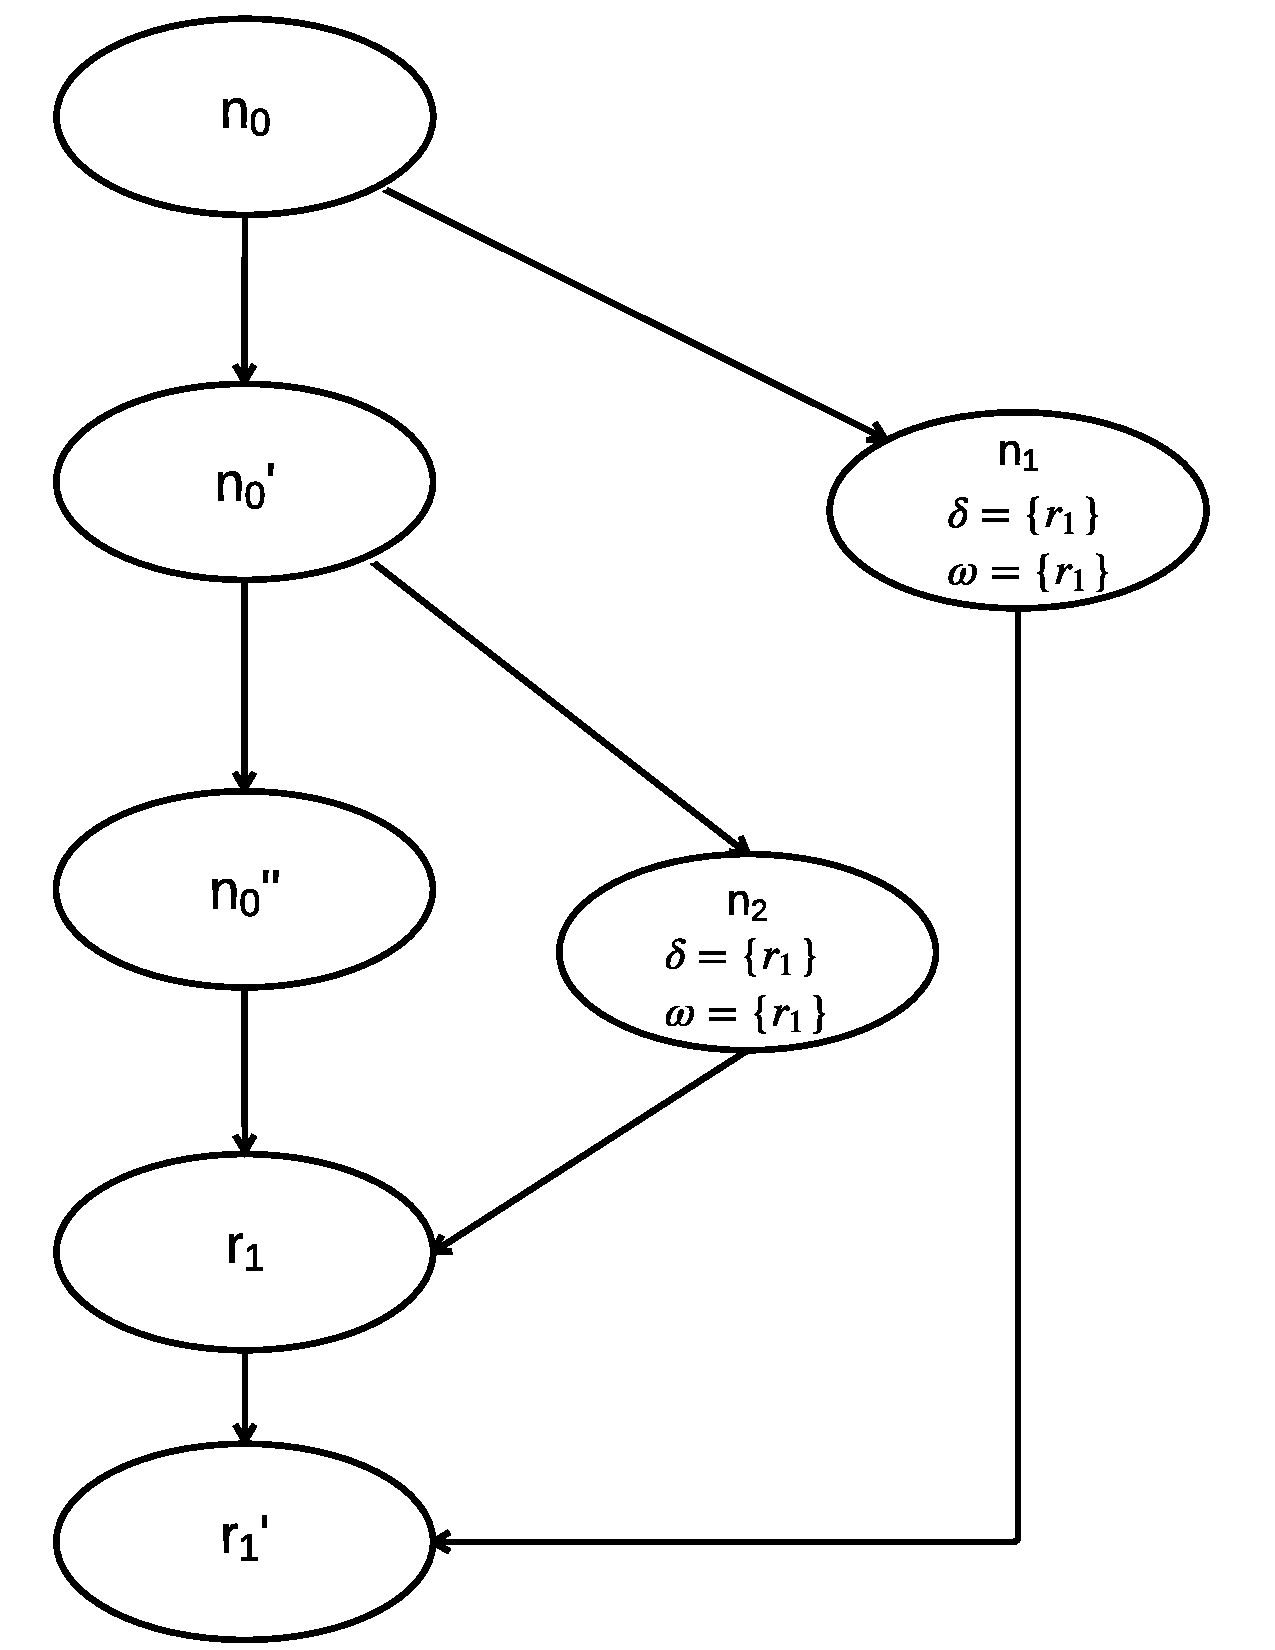
\includegraphics[width=0.5\textwidth]{../figs/Fig3-1.pdf}
    \caption{Computation Graph Example.}
    \label{fig:cg}
\end{figure}

\figref{fig:cg} shows a sample computation graph. In this graph, nodes $n_0$, $n_0'$, $n_0''$, $r_1$, and $r_1'$ belong to task $t_0$. Task $t_0$ spawns two tasks $t_1$ and $t_2$. Node $n_1$ belongs to task $t_1$ and node $n_2$ belongs to task $t_2$. Node $r_1$ and $r_1'$ are join nodes for tasks $t_1$ and $t_2$. 

\begin{algorithm}
\caption{Data Race detection in a computation graph.} \label{algo:drd}
\begin{algorithmic}[1]
\Function{DetectRace}{$Computation Graph \ G$}\label{loc:topo}
\State N := Topologically ordered nodes in G
\For {i in [1, $|N|$]}
\State $n = N[i]$
\For {j in [i+1, $|N|$]} 
\State $n' = N[j]$
\If {$ (n \nprec n') \land (n' \nprec n)$}  \label{loc:path} \label{loc:forall}
	\State \textbf{bool} $\mathtt{rw} = (\delta(n) \cap \omega(n') \neq \emptyset) $
	\State \textbf{bool} $\mathtt{wr} = (\omega(n) \cap \delta(n') \neq \emptyset) $
	\State \textbf{bool} $\mathtt{ww} = (\omega(n) \cap \omega(n') \neq \emptyset)$
		\If {$( \mathtt{rw} \lor \mathtt{wr}  \lor \mathtt{ww} )$} \label{loc:intersection}
			\State \textbf{Report Data Race and Exit} \label{loc:datarace}
		\EndIf
\EndIf
 \EndFor
 \EndFor
\EndFunction  
\end{algorithmic}
\end{algorithm}

Computation graphs can be used to detect data races in parallel programs. Every node in the computation graph represents a block of sequential operations. A computation graph is a partially ordered set of nodes that gives the relationship of the tasks in the program. The transitive closure of the graph gives the reachability of the nodes. The order between any two nodes $n_1$ and $n_2$ is given as $n_1 \prec n_2$, meaning that $n_1$ happens before $n_2$. The operations that may execute in parallel are unordered: $n_1 \nprec n_2$ and $n_2 \nprec n_1$, i. e. $n_1$ does not happen before $n_2$ and $n_2$ does not happen before $n_1$. Once these unordered nodes are identified, the memory accessed by the operations performed in these nodes is checked to detect data races. 

Algorithm \ref{algo:drd} gives the pseudo-code of the algorithm to detect data races in computation graphs. It takes the computation graph as input and reports a data race if an access violation is observed in the graph. The algorithm works as follows. The nodes in the computation graph are added to a topologically sorted set on \lineref{loc:topo}. The $i^{th}$ node in the order is given by N[i]. The nodes are traversed in order and each node is compared to every node that comes later in the topological ordering. \lineref{loc:path} checks if the nodes $n$ and $n'$ are  unordered. If the nodes are unordered, then the sets of memory locations accessed by each node are checked for conflict on \lineref{loc:intersection}. If any of the sets shares an element, then any one of those elements is a location where a data race occurs in the program. A data race is reported by the algorithm on \lineref{loc:datarace}. If the intersecting sets are empty, then the algorithm proceeds to check the next node until either a data race is reported or all the nodes have been verified.

Consider again the example in \figref{fig:cg} with the topological ordering: $n_0$, $n_0'$, $n_0''$, $n_1$, $r_1$, $n_2$, and $r_1'$. Node $n_0$ happens before all other nodes so it cannot data race with anything. The next node in the topological ordering is $n_0'$. It is not ordered relative to $n_1$ so $n_0^\prime$ and $n_1$ are parallel. No race is reported and the analysis proceeds because there are no conflicting accesses made by these nodes. All the nodes are checked one by one in a similar way. The nodes $n_1$ and $n_2$ are unordered since there is no path from $n_1$ to $n_2$ and both are writing to variable $r_1$. Therefore, $\mathtt{ww}$ is set to true and a race is reported for these two nodes on $r_1$.

The algorithm runs in quadratic time for the number of nodes in the computation graph. The topological ordering of nodes can be done in $\mathcal{O}$(N$^2$). When nodes are topologically ordered, reachability of nodes can be checked in $\mathcal{O}$(N) time. Therefore, the time required to check if two nodes are executing in parallel is $\mathcal{O}$(N$^2$). The time required to check the intersection of read or write sets of shared locations is $\mathcal{O}$($m_1 +  m_2$) where $m_1$ and $m_2$ are the sizes of the two sets. ($m_1 + m_2$) is much smaller than N. Therefore, the time complexity of Algorithm \ref{algo:drd}  is $\mathcal{O}$(N$^2$).

\begin{definition} 
\textbf{Sound:} A data race detection algorithm is sound if it does not miss any data race in a program for a given input.
\end{definition}

If the sound algorithm declares a program to be data race free, no race can exist in execution of the program for the given input on any schedule; although, it may reject programs as having data races when in fact they do not. It may under-approximate the set of data race free programs.

\begin{definition}
\textbf{Complete}:  A data race detection algorithm is complete if it does not report data races in programs that are data race free.
\end{definition}

A complete algorithm may accept programs as data race free when in fact they have data races. It may over-approximate the set of data race free programs.

\begin{theorem} \label{thm:graph}
Algorithm \ref{algo:drd} is sound and complete for a given a computation graph $G$.
\end{theorem}

\begin{proof}
The computation graph is a directed acyclic graph. The transitive closure of the graph gives the reachibility relationship of the tasks. The transitive closure is a strict partial order over the nodes of the graph. The data race detection algorithm checks if nodes $n$ and $n^\prime$ in the graph are unordered on Line \ref{loc:forall}. The statements may be executed in parallel by these nodes. The memory accessed by these tasks is compared and a race is reported if a conflict is detected on Line \ref{loc:datarace}. Therefore, when algorithm \ref{algo:drd} declares a computation graph to be data race free, no race can exist in that graph and when a race is reported by the algorithm, there definitely exists two tasks that execute in parallel and have conflicting accesses to a shared variable. Hence, Algorithm \ref{algo:drd} is sound and complete for a given computation graph.
\end{proof}


\chapter{Computation Graphs}
\section{Computation graph creation} \label{sec:cg}

We construct computation graphs by analyzing the execution of task parallel programs defined via a formal model. Our model is derived from Bouajjani and Emmi, who defined the formal model of isolated hierarchical parallel programs to abstractly represent many existing task parallel languages (e.g., Cilk, X10, Chapel, Habanero, etc.) \cite{bouajjani}. However, unlike their model, we do not assume that programs are isolated and do not share memory. Real world task parallel models are not isolated so tasks may share memory (intentionally or otherwise). As much as possible, we mimic the model of Bouajjani and Emmi, but expand their definition in two ways. First, whereas their parallel regions are opaque identifiers, we have them include a single shared variable. Second, in their model tasks have a single set of regions, while in ours in addition to this set, we have two more sets of regions, one where the region variable is readable and the other where the region variable is writable. The rest of this section describes the model in detail, duplicating shared content from their paper.

\subsection{Surface Syntax}

The surface syntax for the language is given in \figref{fig:syntax}. A program \textbf{P} is a sequence of procedures. The procedure name $p$ is taken from a finite set of names \texttt{Proc}. Each procedure has a single $L$-type parameter \texttt{l} taken from a finite set of parameter names \texttt{Vars}. The body of the procedure is inductively defined by $s$. The semantics is abstracted over concrete values and operations, so the possible types of \texttt{l} are not specified nor is the particular expression language, $e$, but assume it includes variables references and Boolean values (\textbf{true} and \textbf{false}). The details of either $L$ or $e$ are never relevant for computation graph construction and are thus omitted. The set of all expressions is given by \texttt{Exprs}. Values are given by the finite set \texttt{Vals} and include at least Boolean values. \texttt{Exprs} contain \texttt{Vals} and the \emph{choice operator} $\star$. 

\begin{figure}
  \begin{center}
\[
  \begin{array}{rcl}
\textbf{P} &::=& (\textbf{proc}~p~(\textbf{var}\ \texttt{l} : L)~s)* \\
\textbf{s} &::=& s;~s \alt \texttt{l} := e \alt \texttt{l}(r)\ := e \\
&\alt& \textbf{skip} \alt  \textbf{assume}~e \\
&\alt& \textbf{if}~e~\textbf{then}~s~\textbf{else}~s \alt \textbf{while}~e~\textbf{do}~s \\
&\alt& \textbf{call}~\texttt{l}\ := p~e~\vec{r_\delta}~\vec{r_\omega} \alt \textbf{return}~e \\
&\alt& \textbf{post}~r \leftarrow p~e~\vec{r}~\vec{r_\delta}~\vec{r_\omega}~d \\
&\alt& \textbf{await}~r \alt \textbf{ewait}~r \\
  \end{array}
\]
  \end{center}
  \caption{The surface syntax for task parallel programs.}
  \vspace{-1em}
  \label{fig:syntax}
\end{figure}

The statements ($s$) of the language denote the behavior of the procedure. Most statements, like the \textbf{if}-statement, \textbf{;}-statement, and \textbf{while}-statement have their typical meaning. Other statements require further explanations.

Statements are divided into the concurrent statements (\textbf{post}-statement, \textbf{await}-statement and \textbf{ewait}-statement) and sequential statements (everything else).  Let \texttt{Regs} be a finite set of region identifiers. Associated with each region $r$ is a single variable referenced in the surface syntax by $\texttt{l}(r)$. A task is posted into a region $r$ by indicating the procedure $p$ for the task with an expression for the local variable value $e$, three lists of regions from $\texttt{Regs}^\ast$ (i.e., the Kleene closure on \texttt{Regs}), and a return value handler $d$. For the region lists, $\vec{r}$ are regions whose ownership is transferred from the parent to the new child task (i.e., the child now owns the tasks in those regions), $\vec{r_\delta}$ are regions in which the new task can read the region variables, and $\vec{r_\omega}$ are regions in which the task can write region variables. Let \texttt{Stmts} be the set of all statements and let $\texttt{Rets} \subseteq (\texttt{Vals} \rightarrow \texttt{Stmts})$ be the set of return value handlers. The handler $d$ associates the return value of the procedure with a user defined statement. 

The \textbf{await} and \textbf{ewait} statements synchronize a task with the sub-ordinate tasks in the indicated region. Intuitively, when a task calls \textbf{await} on region $r$, it is blocked until all the tasks it knows about in $r$ finish execution. Similarly, when a task issues an \textbf{ewait} with region $r$, it is blocked until one task it owns in $r$ completes. The rest of the tasks in the region  $r$ continue their execution normally and are joined when another \textbf{ewait} or \textbf{await} statement is issued by the parent task. A task is termed \emph{completed} when its statement is a \textbf{return}-statement. 

\begin{figure}[h]
  \begin{center}
    \begin{lstlisting}[mathescape=true]
  proc main (var n : int)
  	n := 1;
	post $r_1 \leftarrow p_1~n~\varepsilon~(r_1)~(r_1)~\lambda v.n := n + v$;
	post $r_1 \leftarrow p_2~n~\varepsilon~(r_1)~(r_1)~\lambda v.n := n + v$;
	await $r_1$
  proc $p_1$ (var n : int)
  	$\texttt{l}(r_1) := \texttt{l}(r_1) + n$;
	return (n + 1)
  proc $p_2$ (var n : int)
  	$\texttt{l}(r_1) := \texttt{l}(r_1) + n$;
	return (n + 2)
\end{lstlisting}
  \end{center}
  \vspace{-1em}
  \caption{A simple example of a task parallel program.}
  \label{fig:hj-async-finish}
\end{figure}

The \textbf{assume}-statement blocks a task until its expression $e$ evaluates to \textbf{true}. By way of definition, \textbf{call}, \textbf{return}, \textbf{post}, \textbf{ewait} and \textbf{await} are \emph{inter-procedural} statements. All other statements are \emph{intra-procedural}.

\figref{fig:hj-async-finish} shows a simple example program. The main task posts two new tasks $t_1$ and $t_2$ executing procedures $p_1$ and $p_2$ in region $r_1$. $\varepsilon$ denotes an empty region sequence. The tasks $t_1$ and $t_2$ have access to the variable $r_1$. The $main$ task awaits the completion of $t_1$ and $t_2$. The return value handler of procedure $main$ takes the value returned by the tasks $t_1$ and $t_2$ and updates the value of $n$. The computation graph for this program is that in \figref{fig:cg}.

\subsection{Tree-based Semantics}

The semantics is defined over trees of procedure frames to represent the parallelism in the language rather than stacks which are inherently sequential. That means that the frame of each posted task becomes a child to the parent's frame. The parent-child relationship is transferred appropriately with task passing or when a parent completes without synchronizing with its children. The evolution of the program proceeds by a task either taking an intra-procedural step, posting a new child frame, or removing a frame for a synchronized completed task.

A task $t = \tuple{\ell, s, d, \vec{r_\delta}, \vec{r_\omega}, n}$ is a tuple containing the valuation of the procedure local variable \texttt{l}, along with a statement $s$, a return value handler $d$, a list of regions that it may use for read variables, a list of regions it may use for write variables, and an associated node in the computation graph for this task. When a procedure $p$ is posted as a task, the statement $s$ is the statement defined for the procedure $p$---recall that statements are inductively defined. 

A \emph{tree configuration}, $c = \tuple{t,m}$, is an inductively defined tree with task-labeled vertexes, $t$, and region labeled edges given by the \emph{region valuation} function, $m : \texttt{Regs} \rightarrow \mathbb{M}[\texttt{Configs}]$, where \texttt{Configs} is the set of tree configurations and $\mathbb{M}[\texttt{Configs}]$ are configuration multi-sets. For a given vertex $c = \tuple{t,m}$, $m(r)$ returns the collection of sub-trees connected to the $t$-labeled root by $r$-labeled edges.

The semantics relies on manipulating region valuations for task passing between parents and children. For two region valuations $m_1$ and $m_2$, the notation $m_1 \cup m_2$ is the multi-set union of each valuation. Further, the notation $m\ |_{\vec{r}}$ is the projection of $m$ to the sequence $\vec{r}$ defined as $m\ |_{\vec{r}}(r^\prime) = m(r^\prime)$  when $r^\prime$ is found somewhere in $\vec{r}$, and $m\ |_{\vec{r}}(r^\prime) = \emptyset$ otherwise. 

Let $\llbracket \cdot \rrbracket_e$ be an evaluation function for expressions without any program or region variables such that $\llbracket \star \rrbracket_e = \texttt{Vals}$, and let $\ell(r)$ denote the value of the region variable in $r$. For convenience in the semantics definition, an evaluation function is defined over a task $t$ that enforces the read rights assigned to the task:
\begin{eqnarray*}
  e(t) &=& e(\tuple{\ell, s, d, \vec{r_\delta}, \vec{r_\omega}, n}) \\
  &=& e(\ell, \vec{r_\delta}) \\
  &=& e(\ell, r_0, r_1, \ldots) \\
  &=& \llbracket e[\ell / \texttt{l},\ell(r_0) / \texttt{l}(r_0), \ell(r_1) / \texttt{l}(r_1), \ldots]  \rrbracket_e
  \end{eqnarray*}
If $e[\ell / \texttt{l},\ell(r_0) / \texttt{l}(r_0), \ell(r_1) / \texttt{l}(r_1), \ldots]$ has any free variables, then by definition, $\llbracket e[\ell / \texttt{l},\ell(r_0) / \texttt{l}(r_0), \ell(r_1) / \texttt{l}(r_1), \ldots]  \rrbracket_e$ has no meaning and is undefined (i.e., $e(t) = \emptyset$). e(t) is set-valued, although most expressions evaluate to singletons. As a final convenience for dealing with expressions in the semantics when constructing computation graphs, let the set of regions whose variables appear in $e$ be denoted by $\eta(e)$. 

Contexts are used to further simplify the notation needed to define the semantics.  A \emph{configuration context}, $C$, is a tree with task-labeled vertexes, region-labeled edges and a single $\diamond$-labeled leaf. The notation $C[c]$ denotes the configuration obtained by substituting a configuration $c$ for the unique $\diamond$-labeled leaf of $C$. The configuration isolates individual task transitions (e.g., $C[\tuple{t,m}] \rightarrow C[\tuple{t^\prime,m}]$ denotes an intra-procedural transition on a task). Similarly, a \emph{statement context} is given as $S = \diamond ; s_1; \dots ;s_i$ and $S[s]$ indicates that $\diamond$ is replaced by $s$ where $s$ is the next statement to be executed. A \emph{task statement context}, $T = \tuple{\ell,  S, d, \vec{r_\delta}, \vec{r_\omega}, n}$ is a task with a statement context in place of a statement, and likewise $T[s]$ indicates that $s$ is the next statement to be executed in the task. Like configuration contexts, task statement contexts isolate the statement to be executed (e.g., $C[\tuple{T[s_1],m}] \rightarrow C[\tuple{T[s_2],m}]$ denotes an intra-procedural transition that modifies the statement in some way). For convenience, $e(t)$ is naturally extended to use contexts as indicated by $e(T)$. 

As indicated previously, a task $t$ is completed when its next to be executed statement $s$ is \textbf{return} $e$. The set of possible return-value handler statements for $t$ is $\mathrm{rvh}(t) = \{d(\ell) \mid \ell \in e(T)\}$ given the task's context. By defnition, $\mathrm{rvh}(t) = \emptyset$ when $t$ is not completed or $e(T)$ is undefined. 

The initial condition for a program $\iota = \tuple{p, \ell}$ is an initial procedure $p \in \texttt{Procs}$ and an initial value $\ell \in \texttt{Vals}$. The initial configuration is created from $\iota$ as $c = \tuple{\tuple{\ell, s_p, d, \vec{r_\delta}, \vec{r_\omega}, n}, m}$, where $s_p$ is the statement for the procedure $p$, $d$ is the identity function (i.e., $\lambda v.v$), $\vec{r_\delta}$ list regions whose variables are read by $p$, $\vec{r_\omega}$ lists regions whose variables are written by $p$, $n$ is a fresh node for the computation graph (i.e., $n = \mathrm{fresh}()$), and $\forall r \in \texttt{Regs}, m(r) = \emptyset$.

\begin{comment}
\begin{figure*}
  \begin{center}
    \mprset{flushleft}
    \begin{mathpar}
      \inferrule[Assign Local]
                {
                  \ell^\prime \in e(\ell,\vec{r_\delta}) \\
                  \delta = \delta \cup (n \mapsto \eta(e))
                }
                {
                  \tuple{\ell, S[\texttt{l} := e], d,
                    \vec{r_\delta}, \vec{r_\omega}, n} \rightarrow \\\\
                  \tuple{\ell^\prime, S[\textbf{skip}], d,
                    \vec{r_\delta}, \vec{r_\omega}, n}
                }
      \and
      \inferrule[Assign Region]
                {
                  \ell \in e(T) \\
                  \ell(r) = \ell \\
                  r\ \mathrm{is\ found\ in}\ \vec{r_\omega}(T) \\\\
                  \delta = \delta \cup (n \mapsto \eta(e)) \\
                  \omega = \omega \cup (n \mapsto \{r\})
                }
                {
                  T[\texttt{l}(r)~:=~e] \rightarrow T[\textbf{skip}]
                }
      \and
      \inferrule[Skip]
                {
                }
                {
                  T[\textbf{skip};~s] \rightarrow T[s]
                }
      \and
      \inferrule[Assume]
                {
                  \mathbf{true} \in e(T) \\
                  \mathbf{false} \notin e(T) \\\\
                  \delta = \delta \cup (n \mapsto \eta(e))
                }
                {
                  T[\textbf{assume}~e] \rightarrow T[\textbf{skip}]
                }
      \and
      \inferrule[If-then]
                {
                  \textbf{true} \in e(T) \\
                  \textbf{false} \notin e(T) \\\\
                  \delta = \delta \cup (n \mapsto \eta(e))
                }
                {
                  T[\textbf{if}~e~\textbf{then}~s_1~\textbf{else}~s_2]
                  \rightarrow T[s_1]
                }
      \and
      \inferrule[If-else]
                {
                  \textbf{false} \in e(T) \\
                  \textbf{true} \notin e(T) \\\\
                  \delta = \delta \cup (n \mapsto \eta(e))
                }
                {
                  T[\textbf{if}~e~\textbf{then}~s_1~\textbf{else}~s_2]
                  \rightarrow T[s_2]
                }
      \and
      \inferrule[Do-loop]
                {
                  \textbf{true} \in e(T) \\
                  \textbf{false} \notin e(T) \\\\
                  \delta = \delta \cup (n \mapsto \eta(e))
                }
                {
                  T[\textbf{while}~e~\textbf{do}~s] \rightarrow
                  T[s;~\textbf{while}~e~\textbf{do}~s]
                }
     \and 
     \inferrule[Do-break]
                {
                  \textbf{false} \in e(T) \\
                  \textbf{true} \notin e(T) \\\\
                  \delta = \delta \cup (n \mapsto \eta(e))
                }
                {
                  T[\textbf{while}~e~\textbf{do}~s] \rightarrow
                  T[\textbf{skip}]
                }
    \end{mathpar}
  \end{center}
  \caption{The transition rules for the intra-procedural statements.}
  \label{fig:intra}
\end{figure*}
\end{comment}

The semantics is now given as a set of transition rules relating tree configurations. The rules assume the presence of a global computation graph, $G = \tuple{N, E, \delta, \omega}$, that is updated as part of the transition. The initial graph contains a single node $N = \{n\}$ from the initial configuration, no edges ($E = \emptyset$), and no read/write information ($\delta(n) = \emptyset$ and $\omega(n) = \emptyset$).

\begin{comment}
\figref{fig:intra} lists the intra-procedural transition rules. The rules omit the configuration context since intra-procedural statements do not need the region valuation from the context. The rules define the intra-procedural statements in the usual way. Of note is the update of the computation graph to record any read region variables from expressions or any write region variables from an assignment. The notation, $\delta = \delta \cup (n \mapsto \eta(e))$, is understood to update $\delta$ such that $n$ additionally maps to $\eta(e)$. The notation $\vec{r_\omega}(T)$ in the assign-region rule is used to indicated the read-region vector in the task or task context, $T = \tuple{\ell,  S, d, \vec{r_\delta}, \vec{r_\omega}, n}$. Similar notation is used in other rules to access the tuple.
\end{comment}

\begin{figure*}
  \begin{center}
    \mprset{flushleft}
    \begin{mathpar}
      \inferrule[Call]
                {
                }
                {
                  C[T[\textbf{call}~\texttt{l}\ := p~e~\vec{r_\delta}~\vec{r_\omega}], m] \rightarrow 
                  C[T[\textbf{post}~r_\mathit{call}\leftarrow p~e~\varepsilon~\vec{r_\delta}~\vec{r_\omega}~\lambda v.\texttt{l} := v;~ \textbf{ewait}~r_\mathit{call}], m]
               }
      \and
      \inferrule[Post]
                {
                  n_0^\prime = \mathrm{fresh}() \\
                  n_1 = \mathrm{fresh}() \\\\
                  N = N \cup \{n_0^\prime, n_1\} \\
                  E = E \cup \{\tuple{n_0, n_0^\prime}, \tuple{n_0, n_1}\}\\\\
                  \ell \in e(\ell^\prime,\vec{r_\delta}^\prime) \\
                  \delta = \delta \cup (n_0 \mapsto \eta(e))\\\\
                  m^\prime = (m \setminus m |_{\vec{r}}) \cup
                  (r \mapsto \tuple{
                    \tuple{\ell, s_p, d, \vec{r_\delta}, \vec{r_\omega},n_1},m|_{\vec{r}}})
                }
                {
                  C[\tuple{\ell^\prime,
                      S[\textbf{post}~r \leftarrow p~e~\vec{r}~\vec{r_\delta}~\vec{r_\omega}~d],\vec{r_\delta}^\prime,\vec{r_\omega}^\prime,d^\prime, n_0}, m] \rightarrow \\\\
                  C[\tuple{\ell^\prime,
S[\textbf{skip}],\vec{r_\delta}^\prime,\vec{r_\omega}^\prime,d^\prime, n_0^\prime}, m^\prime]
                }
      \and
      \inferrule[Ewait]
                {
                  n^\prime = \mathrm{fresh}() \\\\
                  N= N \cup \{n^\prime\} \\
                  E = E \cup \{\tuple{n, n^\prime}, \tuple{n(t_2),n^\prime}\} \\\\
                  m_1 = (r \mapsto \tuple{t_2,m_2}) \cup m_1^\prime \\
                  s \in \mathrm{rvh}(t_2) 
                }
                {
                  C[\tuple{\ell,
S[\textbf{ewait}~r],\vec{r_\delta},\vec{r_\omega},d, n}, m_1] \rightarrow \\\\
                  C[\tuple{\ell,
S[s],\vec{r_\delta},\vec{r_\omega},d, n^\prime}, m_1' \cup m_2]
          }
      \and
      \inferrule[Await-next]
                {
                  n^\prime = \mathrm{fresh}() \\\\
                  N= N \cup \{n^\prime\} \\
                  E = E \cup \{\tuple{n, n^\prime}, \tuple{n(t_2),n^\prime}\} \\\\
                  m_1 = (r \mapsto \tuple{t_2,m_2}) \cup m_1^\prime \\
                  s \in \mathrm{rvh}(t_2) 
                }
                {
                  C[\tuple{\ell,
S[\textbf{await}~r],\vec{r_\delta},\vec{r_\omega}, d, n}, m_1] \rightarrow \\\\
                  C[\tuple{\ell,
S[s;~\textbf{await}~r],\vec{r_\delta},\vec{r_\omega},d, n^\prime}, m_1' \cup m_2]
                }
      \and
      \inferrule[Await-done]
                {
                  m(r) = \emptyset
                }
                {
                  C[T_1[\textbf{await}~r] , m] \rightarrow
                  C[T_1[\textbf{skip}], m]
                }
\end{mathpar}
  \end{center}
  \caption{The transition rules for the intra-procedural statements.}
  \label{fig:inter}
    \label{fig:semantics}
\end{figure*}

The intra-procedural transition rules are omitted for space but are defined in the usual way. \figref{fig:inter} shows semantics for the inter-procedural statements. The notation, $\delta = \delta \cup (n \mapsto \eta(e))$, is understood to update $\delta$ such that $n$ additionally maps to $\eta(e)$. A function notation is adopted to access the tuple $T = \tuple{\ell,  S, d, \vec{r_\delta}, \vec{r_\omega}, n}$. For example, $\vec{r_\omega}(T)$ indicates the read-region vector in the task or task context.

The \textbf{call} statement is interpreted as a \textbf{post} followed by \textbf{ewait} on some region $r_{call}$. This region $r_{call}$ is exclusive to the task calling the procedure and cannot be used to post new tasks into this region. A call statement does not allow ownership of any tasks to be passed to the newly created task. The region variables that are available to this task for reading and writing are denoted by $\vec{r_\delta}$ and $\vec{r_\omega}$ respectively.

The \textsc{Post} rule is fired when the task forks to create a new child task that potentially runs in parallel with the parent task. When a task $t_1$ executes a \textbf{post} statement, two fresh nodes $n_0^\prime$ and $n_1$ are added to the graph. Node $n_0^\prime$ represents the statements following \textbf{post} and $n_1$ represents the statements executed by $t_2$. The current node $n_0$ of $t_1$ is connected to $n_0^\prime$ and $n_1$ as shown in \figref{fig:cgcreation}(a). The read set $\delta$ of node $n_0$ is updated to additionally map to the regions in $\eta(e)$ (i.e., the regions referenced in the expression $e$). The current node of $t_1$ changes to $n_0^\prime$ after the transition. The region mapping $m$ of task $t_1$ is updated by removing the configurations of regions whose ownership is passed to the newly created task $t_2$ and adding a new configuration that consists of the task $t_2$ along with the regions it now owns.

The \textsc{Ewait} rule blocks the execution of the currently executing task until a task in the indicated region completes. The choice of completed task, $t_2$, in the region is non-deterministic. A node $n^\prime$ is added to the graph to act as a join node. It captures the subsequent statements of $t_1$ after the \textbf{ewait} statement finishes. The current node $n$ of task $t_1$ and the current node of task $t_2$, denoted by $n(t_2)$ are connected to $n^\prime$ as shown in \figref{fig:cgcreation}(b). The configuration ($r \mapsto \tuple{t_2,m_2}$) is removed from the region valuation $m$ of $t_1$. After the transition, the current node of task $t_1$ is changed to $n^\prime$.  The task $t_1$ is resumed with a return value handler for the completed task ($\mathrm{rvh}(t_2)$) before continuing with its next statement.

The \textsc{Await-Next} rule blocks the execution of the currently executing task $t_1$ until 
%all the tasks whose handles are stored in region $r$ that the task $t_1$ owns are executed to completion. 
all the tasks owned by $t_1$ whose handles are stored in region $r$ complete execution.
The rule is implemented recursively by removing one task from the region at a time and then inserting another \textbf{await}-statement on the same region. A join node $n^\prime$ is added to the graph, the current nodes of $t_1$ and $t_2$ are connected to $n^\prime$ as shown in \figref{fig:cgcreation}(b) and the current node of $t_1$ is changed to $n^\prime$. When task $t_2$ returns a value to $t_1$, $t_1$ executes the statement from the return value handler $\mathrm{rvh}(t_2)$. The \textsc{Await-Done} rule terminates recursion when the region is empty. 

\begin{figure}
  \begin{center}
     \subfigure[Task creation.]{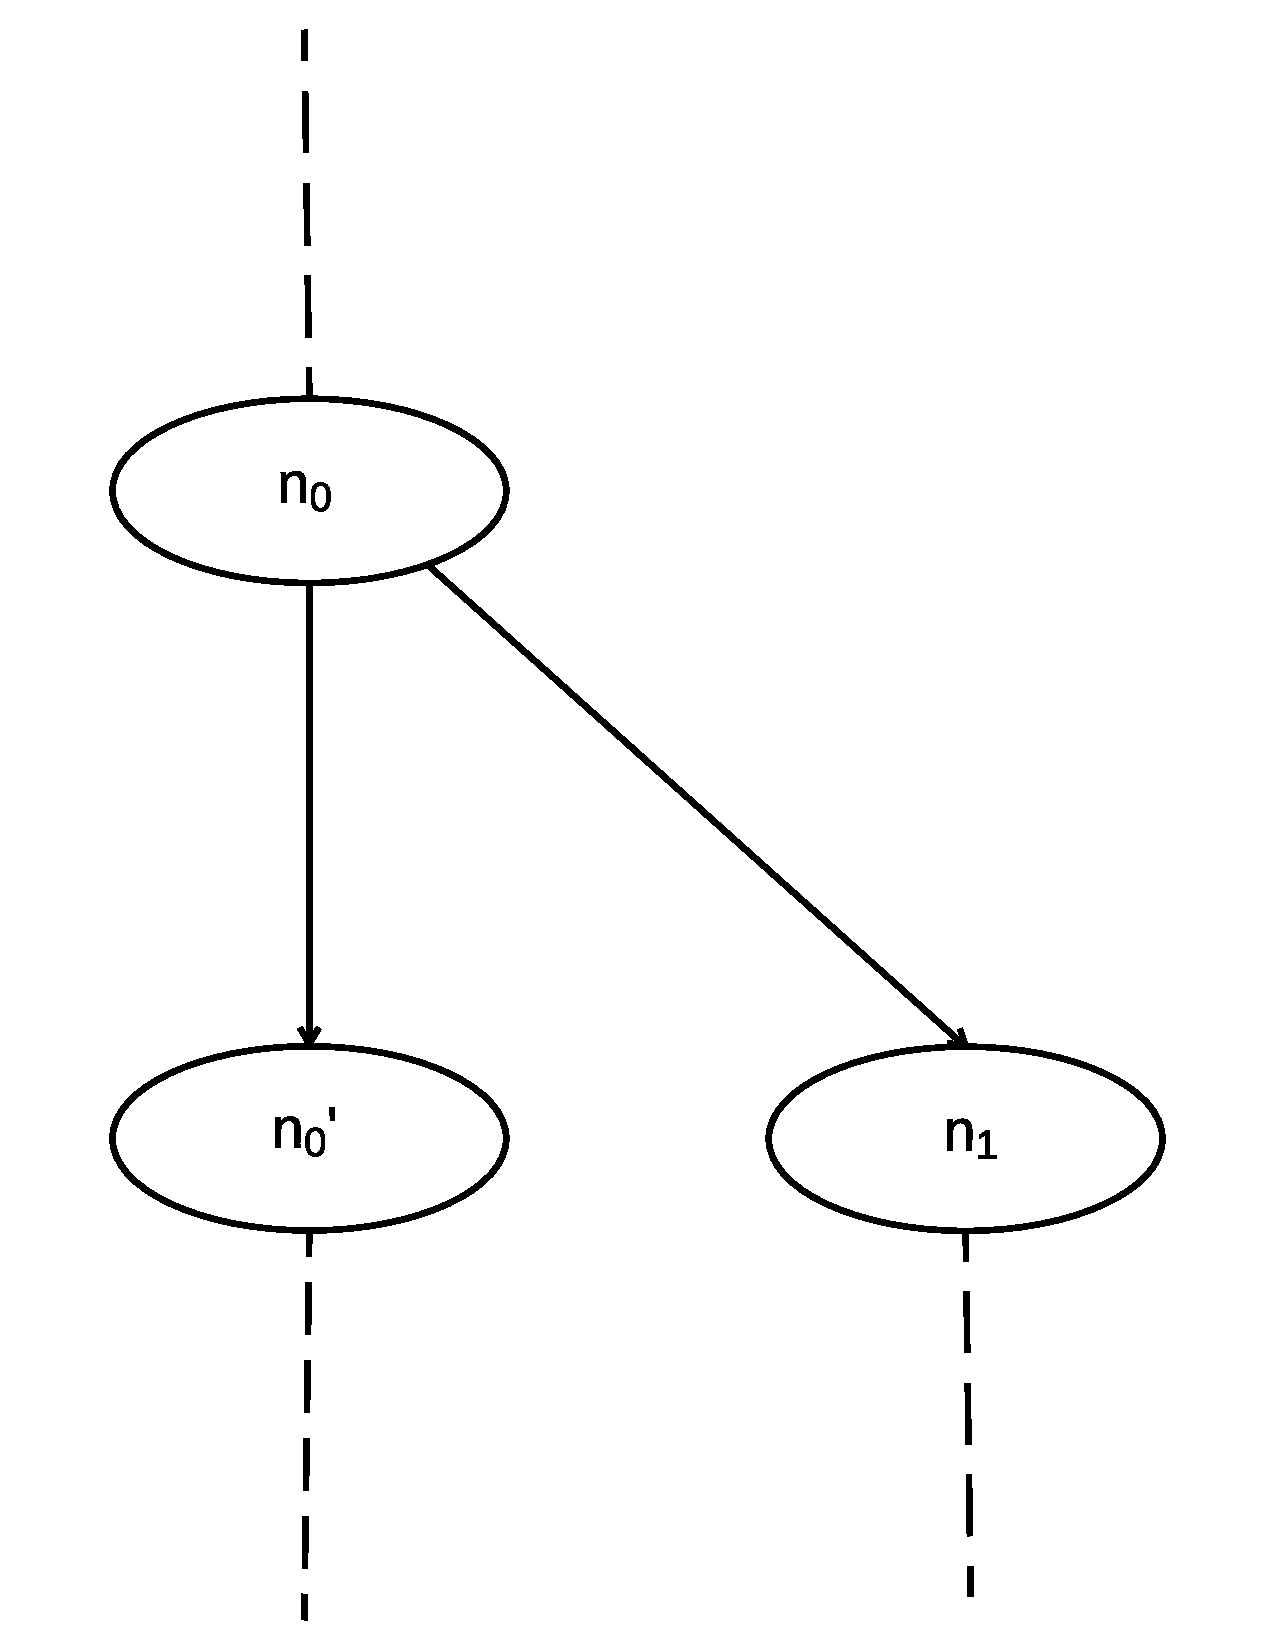
\includegraphics[scale=0.2]{../figs/Fig1-a.pdf}}
     \subfigure[Task synchronization.]{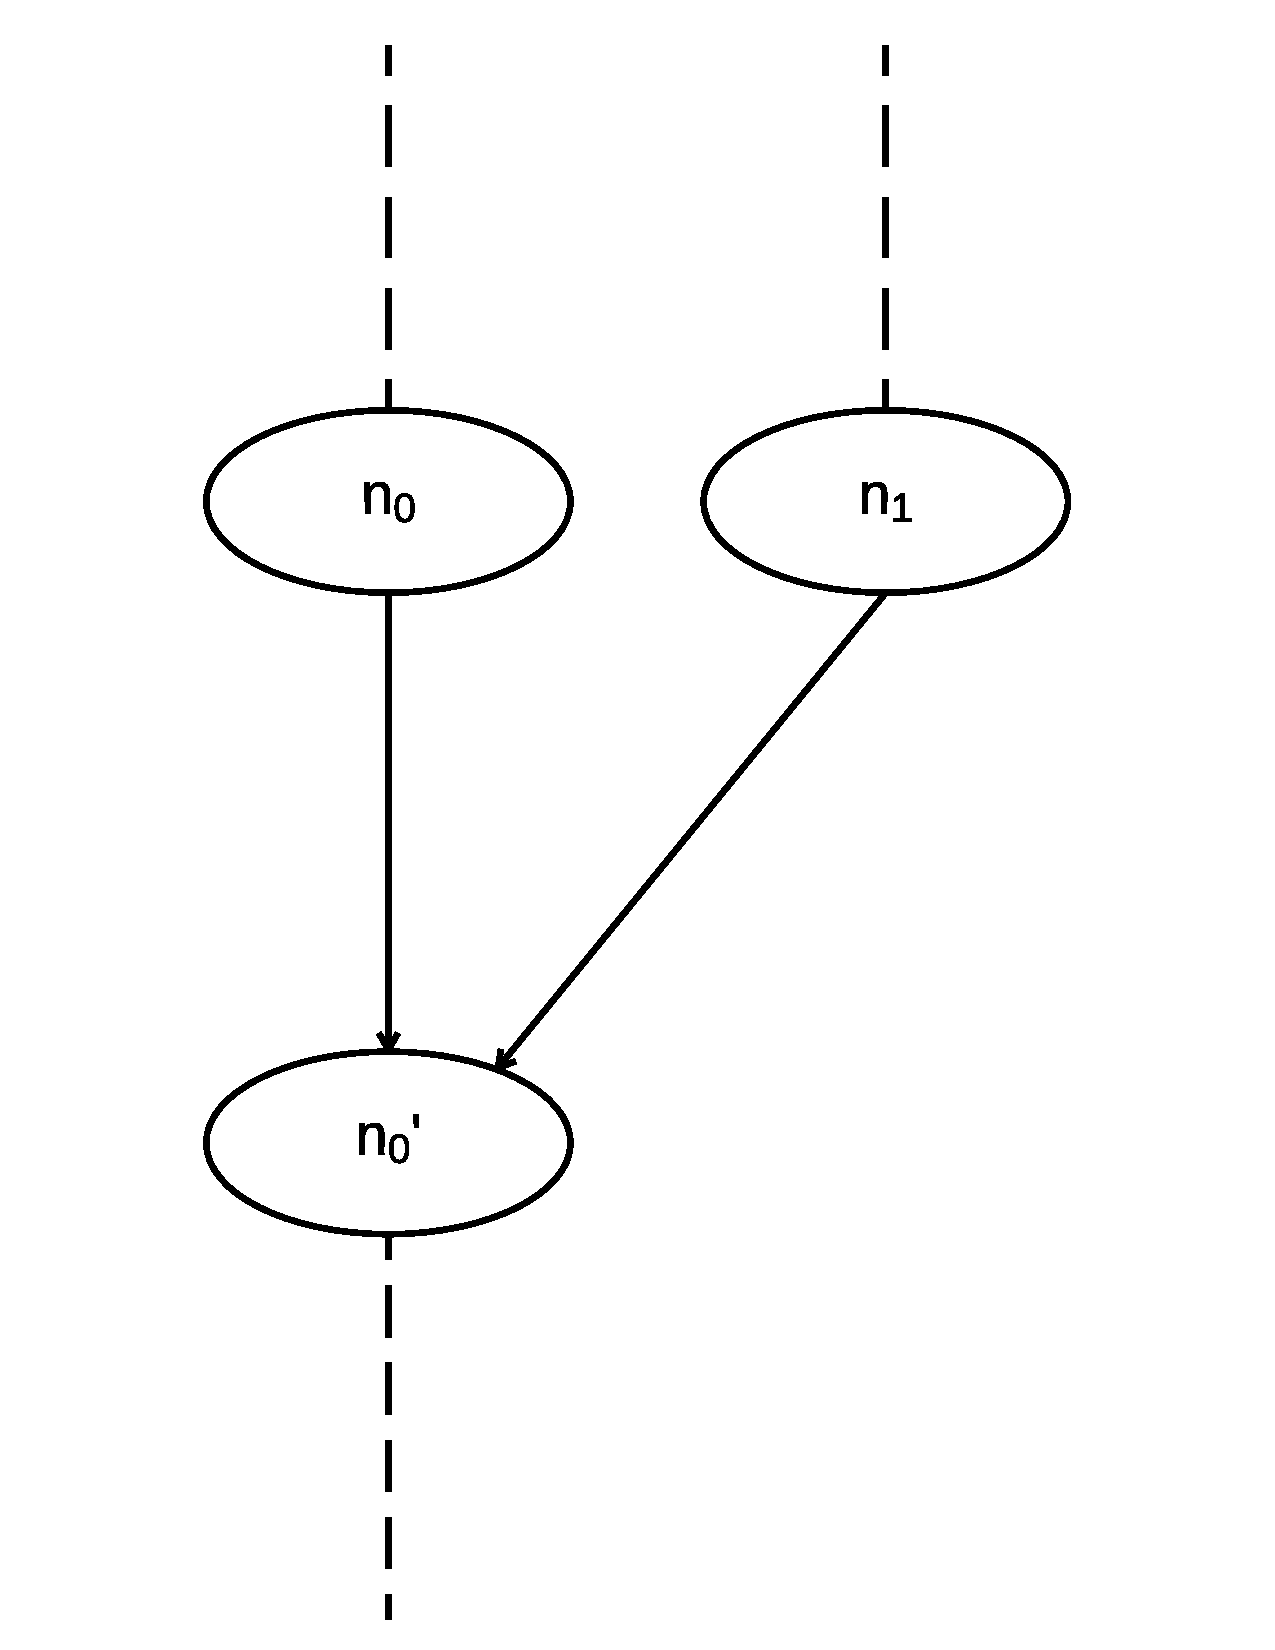
\includegraphics[scale=0.2]{../figs/Fig1-b.pdf}}
  \caption{Steps involved in computation graph creation.}
  \vspace{-1em}
   \label{fig:cgcreation}
   \end{center}
\end{figure}

The computation graph for the example in \figref{fig:hj-async-finish} is presented in \figref{fig:cg}. The order of synchronization of tasks $t_1$ and $t_2$ affects the value of the variable $r_1$ in the $main$ task. The return value handlers of the tasks get executed in different orders under different program schedules. This makes the output of the program non-deterministic. In a schedule where task $t_1$ joins $main$ task before $t_2$, the value of $n$ at the end of program execution is 3 and in a schedule where task $t_2$ joins $main$ task before $t_1$, the value of $r_1$ is 2.

\begin{theorem}
Algorithm \ref{algo:drd} is complete for a task parallel program with a given input.
\end{theorem}
\begin{comment}
\begin{proof}

%Proof is available in the longer version of this paper.


The semantics described in \figref{fig:semantics} show how a computation graph is built for a task parallel program from an observed program execution. The nodes in the graph depict the correct partial order between the tasks in the program. Theorem \ref{thm:graph} shows that Algorithm \ref{algo:drd} is sound and complete for a given computation graph. A task parallel program can have different computation graphs based on the schedule followed by the tasks during the program execution. If Algorithm \ref{algo:drd} does not report a race for a computation graph obtained from some execution of the program, data races may still be observed under some other program schedule. Therefore, Algorithm \ref{algo:drd} is complete for a task parallel program with a given input.

\end{proof}
\end{comment}

\chapter{Structured Parallel Languages}
\section{A Deterministic Fragment of the Model}
\label{sec:otf-drd}
This section defines a deterministic fragment of the task parallel language such that a computation graph from a single execution is sufficient to prove or disprove data-race. In other words, data-race detection using \algoref{algo:drd} on the computation graph from an single execution of a program in this fragment is both sound and complete meaning that it neither under-approximates (sound) nor over-approximates (complete) the set of data-race free programs. The fragment is defined by the following language restrictions:
\begin{compactitem}
\item Passing ownership of tasks from a parent to a child task is not allowed. 
\item Tasks whose return value handlers side effect can be posted in single-task regions only (i.e., regions that contain only a single task). A side-effect of a return value handler can be a change in the state of either the local variable or a region variable. 
\item All the tasks are joined to the main task at the end of the program execution. This is ensured by having the initial program configuration as \tuple{$T[\textbf{post} $ r_0 \leftarrow p_0~e~\varepsilon~\vec{r}~\vec{r}~\lambda$v.v; $\textbf{await}~r_0; \textbf{await}~r_1; \ldots], m_0} on some procedure $p_0$, $\vec{r}$ is the region sequence containing all regions and $\forall r \in \mathtt{Regs},$ $m_0(r) = \emptyset$
\end{compactitem}
\figref{fig:hj-async-fin} is an example, with a data-race, from the equivalent fragment in the Habanero model to show the relationship to real-world programming languages. 

In Habanero, the \textbf{async} construct creates a new asynchronous task that runs in parallel with the parent task. The \textbf{finish} construct is used to collectively synchronize children tasks with their parent task. The \textbf{finish} $s$ statement causes the parent task to execute $s$ and then wait until all tasks created inside the finish-block have completed. The future construct lets tasks return values to other tasks with the operation \texttt{f.get()} that blocks until the task associated with $f$ completes. 

\begin{figure}
  \begin{center}
\begin{lstlisting}
public class Example1{
   static int x = 0;
   public static void main(String[] args) {
      finish {
         async { //Task1
           x = x + 1;
         }
         finish{
            async { //Task2
              x = x + 2;
            }
         }
      }
      future f = async { //Task3
                    return 5;
                 }
      x = f.get();
   }
}
\end{lstlisting}
  \end{center}
%  \vspace{-2em}
  \caption{An example of a Habanero Java Program.}
%   \vspace{-2em}
  \label{fig:hj-async-fin}
\end{figure}

\begin{figure}
  \begin{center}
\begin{lstlisting}[mathescape=true]
  proc $main$ (var n : int)
  	$\texttt{l}(r_1) := 0;$
	post $r_1 \leftarrow p_1~0~\varepsilon~\vec{r}~\vec{r}~\lambda n.n$;
	post $r_2 \leftarrow p_2~0~\varepsilon~\vec{r}~\vec{r}~\lambda n.n$;
	await $r_2$;
	await $r_1$;
	post $r_3 \leftarrow p_3~0~\varepsilon~\vec{r}~\vec{r}~\lambda n. \texttt{l}(r_1) := 5$;
	ewait $r_3$;	
  proc $p_1$ (var n : int)
  	$\texttt{l}(r_1) := \texttt{l}(r_1) + 1$
  proc $p_2$ (var n : int)
  	$\texttt{l}(r_1) := \texttt{l}(r_1) + 2$
  proc $p_3$ (var n : int)
  	return 5
\end{lstlisting}
  \end{center}
%    \vspace{-2em}
  \caption{Converted version of the Habanero Java program from \figref{fig:hj-async-fin}.}
%        \vspace{-1em}
  \label{fig:hj-async-fin-converted}
\end{figure}

\figref{fig:hj-async-fin-converted} is the equivalent program in the model in this presentation. The procedure $main$ posts task from the outer finish block to region $r_1$ and tasks from the inner finish block to region $r_2$. Since, the inner finish block completes execution first, \textbf{await} on region $r_2$ is called before $r_1$. The future posts a task to region $r_3$ followed by an \textbf{ewait} on $r_3$.

Let $\mathcal{G}( P )$ return the set of computation graphs from all possible schedules of the program $P$ from the deterministic fragment of the model, and let $\mathrm{DRF}( G )$ return true if \algoref{algo:drd} reports the graph to be data race free. 

\begin{lemma} 
\label{lem:drf}
 $(\exists G \in \mathcal{G}( P ),\ \mathrm{DRF}( G )) \rightarrow (\forall G \in \mathcal{G}( P ),\ \mathrm{DRF}( G ))$ 
\end{lemma}

The proof is omitted for space (as are the other non-trivial proofs), but the lemma states that if data-race is not detected in an observed execution of a program from the deterministic fragment, then all other possible executions are data-race free as well; in other words, programs from the fragment are deterministic.
Habanero makes this same claim but does not prove it \cite{cave2011habanero}. The corollary regarding data-race programs and the following theorem are trivial from \lemmaref{lem:drf}.

\begin{corollary}\label{cor:drf}
$(\exists G \in \mathcal{G}( P ),\ \neg\mathrm{DRF}( G )) \rightarrow (\forall G \in \mathcal{G}( P ),\ \mathrm{DRF}( G ))$ 
\end{corollary}

\begin{theorem} \label{thm:strcutured-par-progs}
Using the tree semantics with Algorithm \ref{algo:drd} to detect data-race in the resulting computation graph is sound and complete for a task parallel program with a given input when that program is in the deterministic fragment of the language.
\end{theorem}


\chapter{On-the-fly data race detection}
\section{Model Checking}

Programs that use mutual exclusion to protect accesses to shared variables introduce non-determinism as different access orders in the critical sections may lead to different computation graphs. Model checking can be used to enumerate each of these computation graphs. The task parallel language is extended to model mutual exclusion with a new statement: $\textbf{isolated}~s$.
The statement performs $s$ in mutual exclusion of any other isolated statements. The semantics with the computation graph construction is in \figref{fig:isol-semantics}. The isolation is accomplished by creating a new global variable \textit{last} to track the last node in the computation graph belonging to an isolated statement, by adding to the task context a counter initialized to zero to count the number of nested isolated contexts, and with a new keyword for the rewrite rules: \textbf{isolated-end}. 

\begin{figure*}
  \begin{center}
    \mprset{flushleft}
    \begin{mathpar}
     \and
      \inferrule[Isolated]
                {
				  \mathrm{canIsolate(C)} = \mathit{true} \\
                  n^\prime = \mathrm{fresh}() \\
                  N = N \cup \{n^\prime\} \\
                  E = E \cup \{\tuple{n, n^\prime},  \tuple{\mathit{last},n^\prime}\}\\
                }
{C[\tuple{\ell^\prime,S[\textbf{isolated}~s],\vec{r_\delta}^\prime,\vec{r_\omega}^\prime,d^\prime, n, 0}, m] \rightarrow
                  C[\tuple{\ell^\prime,
				   S[s; \textbf{isolated-end}],\vec{r_\delta}^\prime,\vec{r_\omega}^\prime,d^\prime, n^\prime, 1}, m]
                }
\and
      \inferrule[Isolated-Nested]
                {\mathit{iso} > 0 \\
                  \mathit{iso}^\prime = \mathit{iso} + 1
                }
{C[\tuple{\ell^\prime,S[\textbf{isolated}~s],\vec{r_\delta}^\prime,\vec{r_\omega}^\prime,d^\prime, n, \mathit{iso}}, m] \rightarrow
                  C[\tuple{\ell^\prime,
				   S[s; \textbf{isolated-end}],\vec{r_\delta}^\prime,\vec{r_\omega}^\prime,d^\prime, n, \mathit{iso}^\prime}, m]
}
\and
      \inferrule[Isolated-End-Nested]
                {\mathit{iso} > 1 \\
                  \mathit{iso}^\prime = \mathit{iso} - 1
                }
{C[\tuple{\ell^\prime,S[\textbf{isolated-end}],\vec{r_\delta}^\prime,\vec{r_\omega}^\prime,d^\prime, n, \mathit{iso}}, m] \rightarrow
                  C[\tuple{\ell^\prime,
				   S[\textbf{skip}],\vec{r_\delta}^\prime,\vec{r_\omega}^\prime,d^\prime, n, \mathit{iso}^\prime}, m]
                }
\and
      \inferrule[Isolated-End]
                {
                  n^\prime = \mathrm{fresh()}\\
                  \mathit{last} = n \\
                  N = N \cup \{n^\prime\} \\
                  E = E \cup \{\tuple{n, n^\prime}\}
                }
{C[\tuple{\ell^\prime,S[\textbf{isolated-end}],\vec{r_\delta}^\prime,\vec{r_\omega}^\prime,d^\prime, n, 1}, m] \rightarrow
                  C[\tuple{\ell^\prime,
				   S[\textbf{skip}],\vec{r_\delta}^\prime,\vec{r_\omega}^\prime,d^\prime, n^\prime,0}, m]
                }

\end{mathpar}
  \end{center}
  \caption{The transition rules for isolated statements.}
  \label{fig:isol-semantics}
\end{figure*}

Let $\mathrm{canIsolate}(C)$ be a function over configurations to Boolean that returns true for a configuration tree if all the task counters are 0; otherwise it returns false. If no other isolated statements are running, then the \textsc{Isolated} rule increments the task counter to indicate isolation and inserts after the isolated statement $\mathit{s}$ the new \textbf{isolated-end} keyword. The computation graph gets a new node to track accesses in the isolated statement with an appropriate edge from the previous node. A sequencing edge from $\mathit{last}$ is also added so the previous isolated statement happens before this new isolated statement. As a note, $\mathit{last}$ is initialized to an empty node when execution starts. The \textsc{Isolated-Nested} rule simply increments the counter if the task is already in isolation.

The \textsc{Isolated-End-Nested} rule processes the new \textbf{isolated-end} keyword and decrements the counter. When the counter reaches the outer-most isolated context, the \textsc{Isolated-End} rule creates a new node in the computation graph to denote the end of isolation, and it updates $\mathit{last}$ to properly sequence any future isolation. As a note, the on-the-fly data race detection is modified to not reduce sub-graphs with isolation.

Algorithm \ref{algo:isolated} presents a scheduling algorithm to enumerate all computation graphs resulting from isolation for model checking \cite{mercer2015model}. The algorithm considers a simplified state of the program with $\mathtt{Regs}$ being the set of region variables that are shared among the tasks, $\mathtt{Tasks}$ being the set of tasks, $t$ being a task, and $R$ being the set of runnable tasks. The algorithm also implements \emph{sequential semantics}, or depth-first semantics, where only one task runs at a time and that task runs until it waits, completes, or isolates at which time a scheduling choice is made. Sequential semantics are viable by \lemmaref{lem:drf} and \corref{cor:drf} that establish independence in the computation graph and execution schedule in the absence of data races. 

\begin{algorithm}
\caption{Scheduling algorithm for Isolated blocks} \label{algo:isolated}
\begin{algorithmic}[1]
  \Function{schedule}{$t$, $\mathtt{Regs}$, $\mathtt{Tasks}$}
  \State \texttt{loop}:\ ($\mathtt{Regs}$, $\mathtt{Tasks}$) $:=$ \texttt{run}($t$, $\mathtt{Regs}$, $\mathtt{Tasks}$)\label{loc:run}
  \State $s :=$ \texttt{status}($t$)
  \State $R :=$ \texttt{runnable}($\mathtt{Tasks}$)
  \If{ $s =$ ISOLATED}\label{loc:entry:isolated}
  \ForAll{$t_i \in R$}\label{loc:prsched}
  \State \texttt{schedule}($t_i$, $\mathtt{Regs}$, $\mathtt{Tasks}$)
  \EndFor
  \Else
  \State $t_i$ := \texttt{random}($R$)\label{loc:rand}
  \State \texttt{schedule}($t_i$, $\mathtt{Regs}$, $\mathtt{Tasks}$)
  \EndIf
  \EndFunction
\end{algorithmic}
\end{algorithm}


Line 2 updates the region variables and pool of tasks by running task $t$ until it exits, waits, or reaches an \textbf{isolated}-construct. The function \texttt{status} on Line 3 returns the status of the task $t$. On Line 4, the function \texttt{runnable} is used to obtain a list of all the tasks that can be run from the pool of all tasks. If the status of the currently running task $t$ becomes ISOLATED (i.e., the task encounters an \textbf{isolated} construct), the task is preempted and all the tasks that are runnable, including the task that is trying to isolate, are scheduled by the runtime. When the task completes, a new task is randomly selected from the set of runnable tasks.

\begin{comment}
\begin{figure}
  \begin{center}
    \begin{lstlisting}[mathescape=true]
  proc main(var n : int)
  	n := 1;
  	post $r_1 \leftarrow p_1~n~\varepsilon~\{r_1\}~\{r_1\}~\lambda v. n := n + v$;
  	post $r_1 \leftarrow p_2~n~\varepsilon~\{r_1\}~\{r_1\}~\lambda v. n := n + v$;
  	await $r_1$
 proc $p_1$(var n : int)
 	isolated $\texttt{l}(r_1) := n + 1$
 proc $p_2$(var n : int)
	isolated if $(\texttt{l}(r_1) = n)$ then
	  	post $r_1 \leftarrow p_3~n~\varepsilon~\{r_1\}~\{r_1\}~\lambda v. n := n + v$;
	else
		$\texttt{l}(r_1) := n - 1$
 proc $p_3$(var n : int)
	$\texttt{l}(r_1) := n+2$
\end{lstlisting}
  \end{center}
  \vspace{-1em}
  \caption{Parallel Program with Mutual exclusion.}
  \vspace{-1em}
  \label{fig:hj-isolated}
\end{figure}

\begin{figure}
  \centering
  \subfigure[p2 runs before p1.]{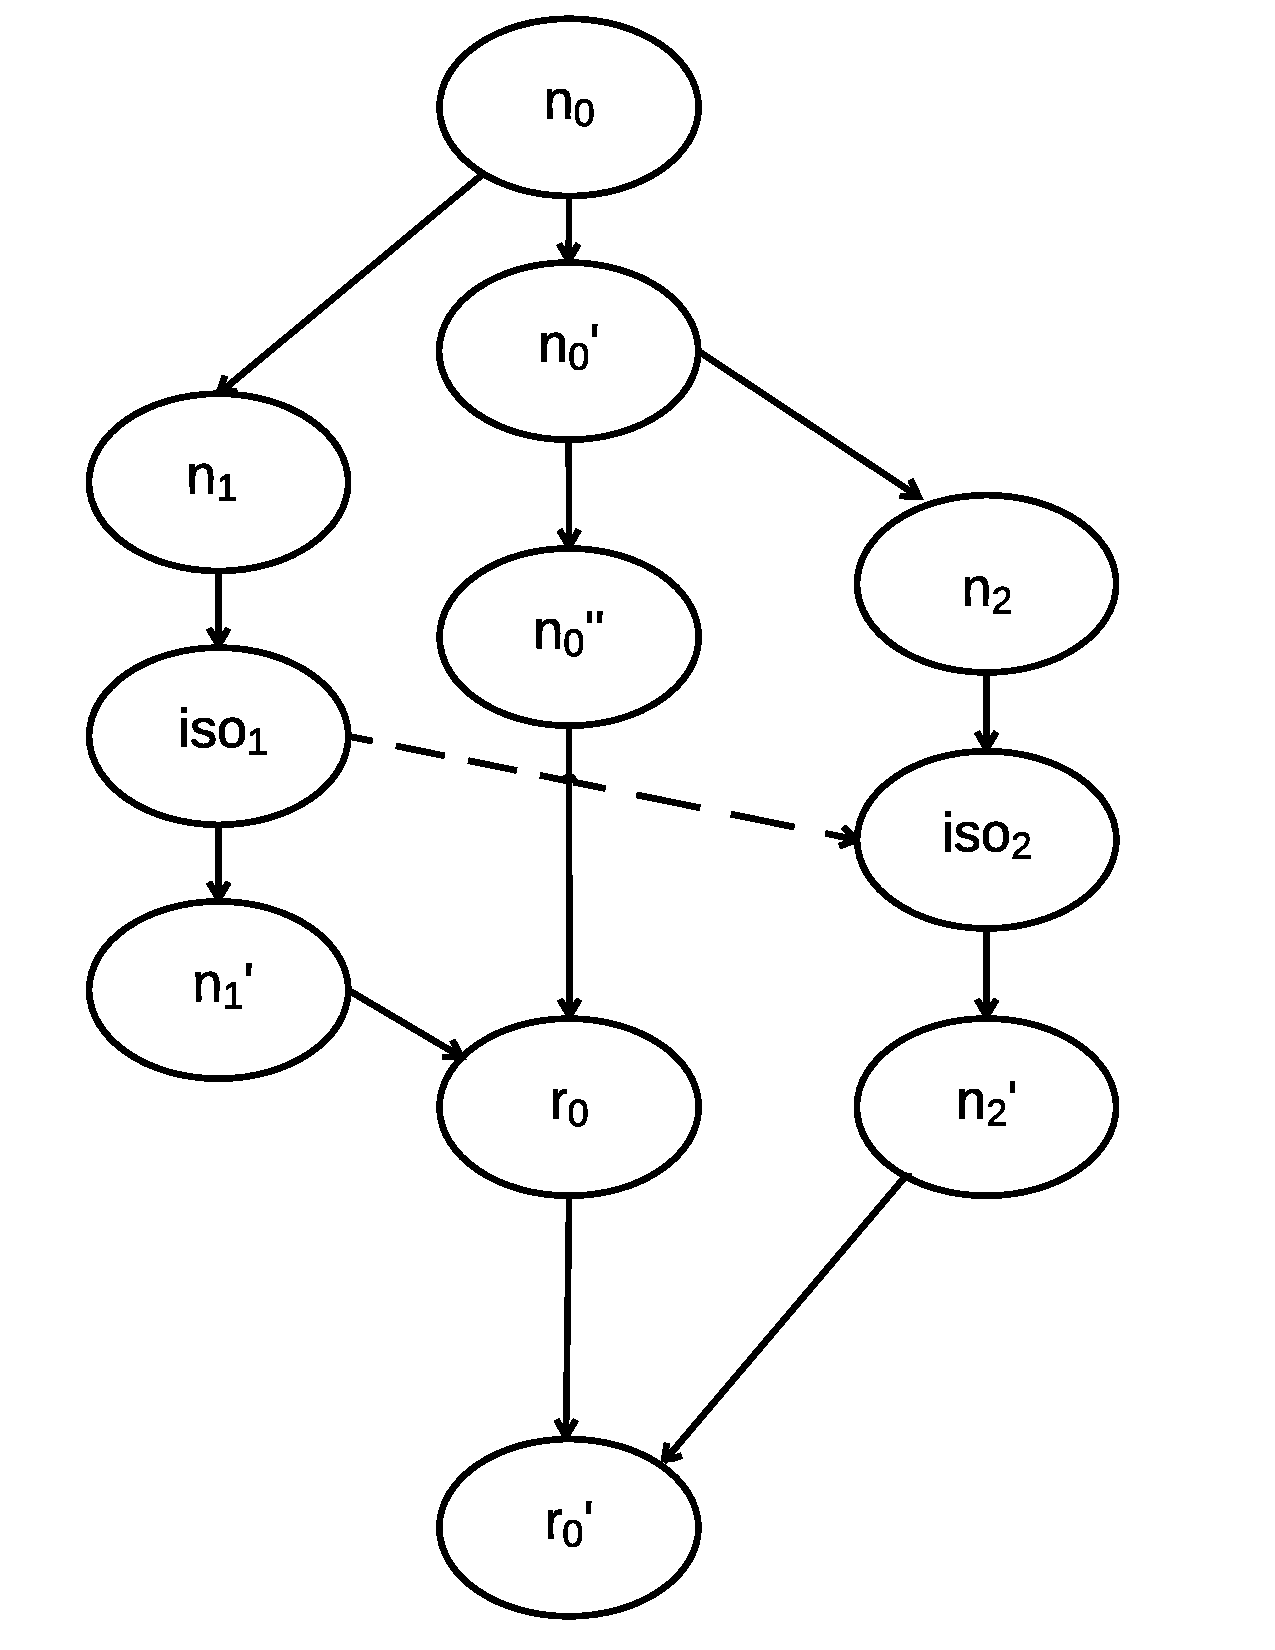
\includegraphics[scale=0.2]{../figs/Fig5-a.pdf}}
  \subfigure[p1 runs before p2.]{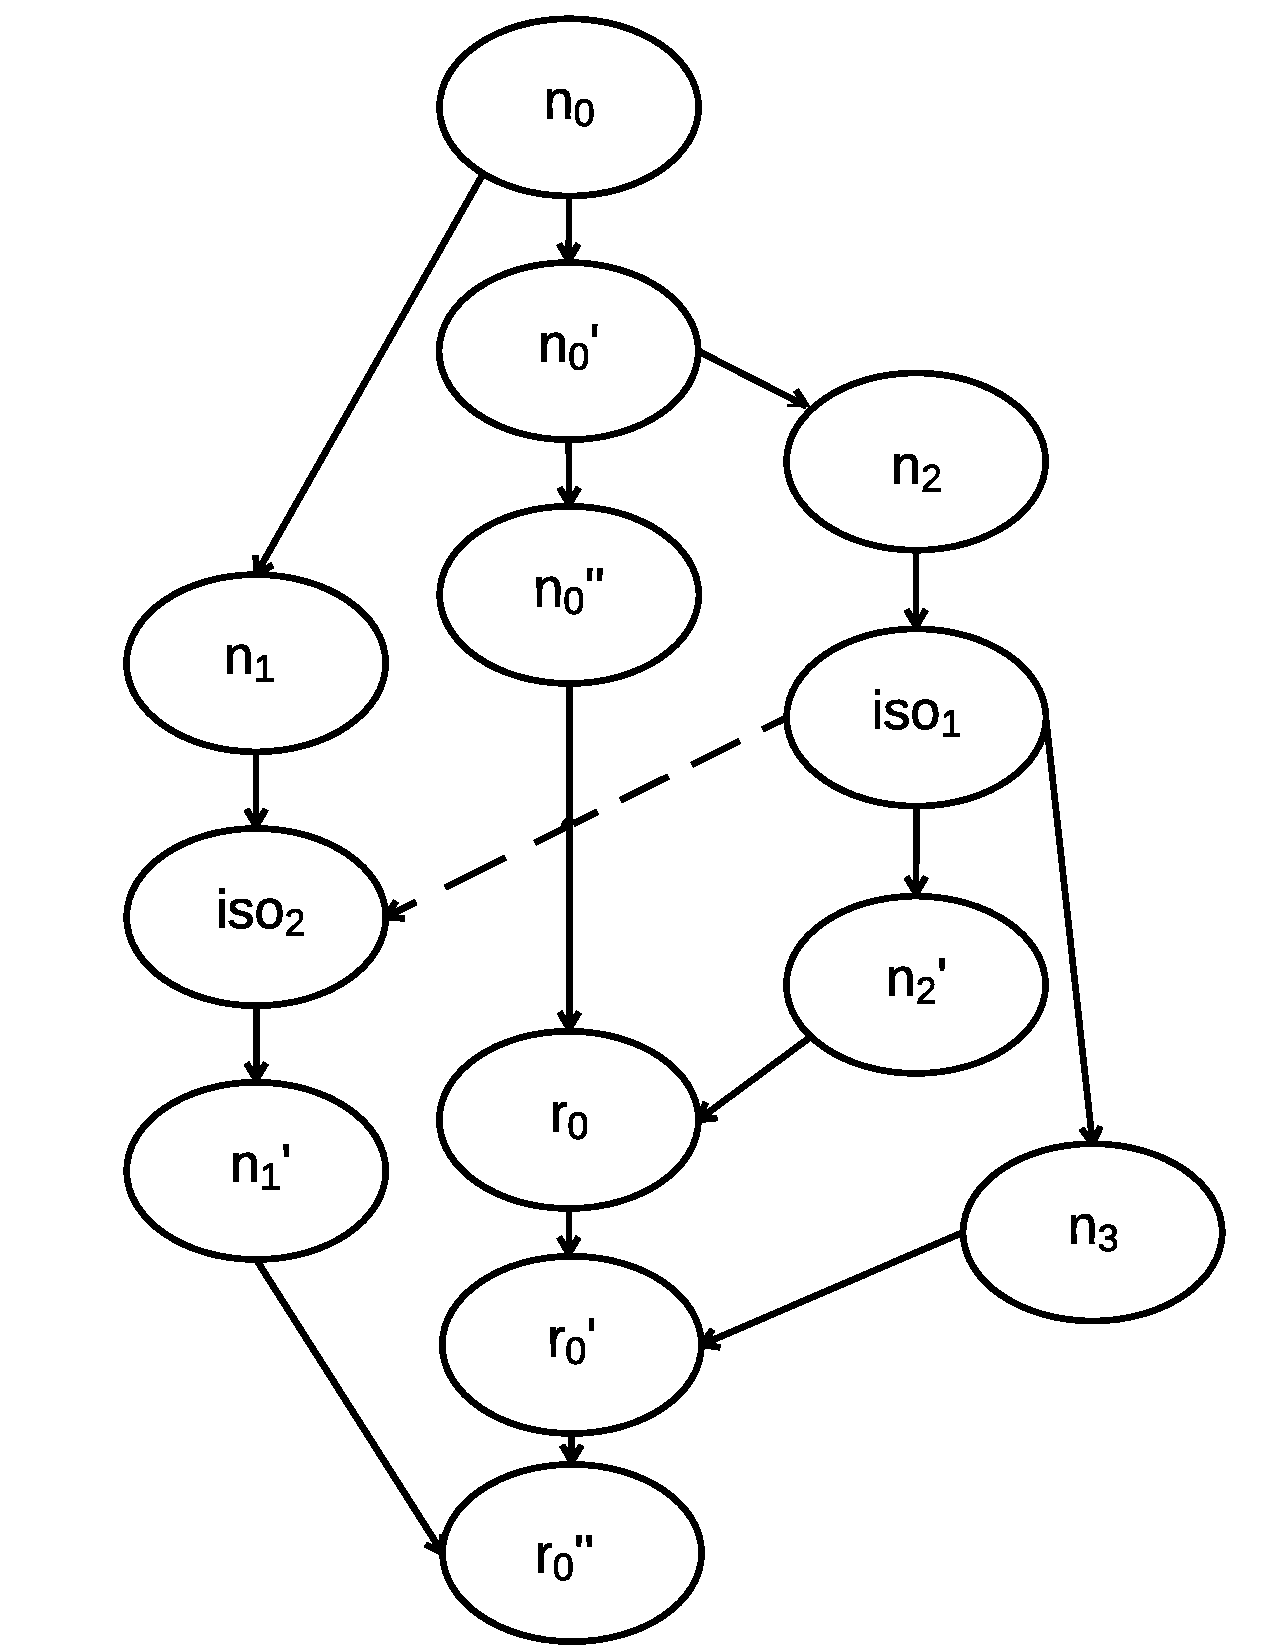
\includegraphics[scale=0.2]{../figs/Fig5-b.pdf}}
  \caption{Computation graphs of example in \figref{fig:hj-isolated}}
  \vspace{-1em}
   \label{fig:cg-isolated}
\end{figure}

For the example in \figref{fig:hj-isolated}, two different computation graph structures can be formed based on the order of execution of isolated blocks. The computation graphs are shown in \figref{fig:cg-isolated}. If the scheduler runs the isolated section of task $t_1$ first, the computation graph in \figref{fig:cg-isolated}(a) is formed. Task $t_1$ changes the values of shared variable $r_1$ to 2. Hence, when task $t_2$ executes its isolated section, the if-condition fails and an additional task is not spawned by $t_2$. If the scheduler runs task $t_2$ first, the computation graph of \figref{fig:cg-isolated}(b) is formed. In this schedule, task $t_2$ executes its isolated section first. Since the value of variable $r_1$ is 1, the if-condition is met and a new task is created by $t_2$.
\end{comment}

\begin{theorem}
Using isolated semantics with \algoref{algo:drd} to check a constructed computation graph and using \algoref{algo:isolated} to enumerate all feasible computation graphs for a program with a given input is sound and complete.
%\algoref{algo:drd} is sound and complete for structured parallel programs with mutual exclusion.
\end{theorem}

\begin{comment}
\begin{proof}
%Theorem \ref{thm:strcutured-par-progs} states that Algorithm \ref{algo:drd} is sound and complete for structured parallel programs that do not contain isolated sections. If mutual exclusion is present, Algorithm \ref{algo:drd} does not remain sound since different computation graph structures can be formed for such programs. Algorithm \ref{algo:isolated} helps to enumerate all such computation graph structures. Therefore, the data race detection using Algorithm \ref{algo:drd} becomes sound and complete when it is used along with Algorithm \ref{algo:isolated} for structured parallel programs that have mutual exclusion.
From \thmref{thm:strcutured-par-progs} and \algoref{algo:isolated}, \algoref{algo:drd} is sound and complete for structured parallel programs with mutual exclusion.
\end{proof}
\end{comment}


\chapter{Mutual Exclusion}
\section{Mutual Exclusion} \label{sec:mutex}

Data races in parallel programs lead to non-deterministic behavior of programs. Therefore, data races are termed as errors. When access to a shared variable is protected by a lock, there is a programmer intended race on the variable. When these accesses are not ordered by the programmer, the output of the program is becomes non-deterministic. This behavior, however, is expected by the programmer. 

Programs with data races can have different computation graph structures based on the schedule of tasks in the runtime (i.e., different update orders may result in different control flow paths). Similarly, when shared memory accesses are protected using locks, different computation graph structures can be observed based on the order in which the tasks access the protected shared variable. To ensure that a program in which tasks have mutually exclusive access to some shared variable does not have any unintended race, all the computation graph structures that can result from different schedules over the protected shared variable access have to be enumerated and analyzed.

\begin{figure}[h]
\vspace{-1em}
  \begin{center}
\[
  \begin{array}{rcl}
\textbf{s} &::=& \textbf{isolated}~\texttt{l}\ := p~e~\vec{r_\delta}~\vec{r_\omega}
  \end{array}
\]
  \end{center}
  \caption{The surface syntax for task parallel programs extended with isolated}
  \label{fig:syntax-iso}
\end{figure}

The surface syntax of task parallel languages has been extended to include isolated statements as shown in \figref{fig:syntax-iso}. 
The \textbf{isolated} statement runs procedure $p$ in mutual exclusion with any other \textbf{isolated} procedure.

\begin{figure*}
  \begin{center}
    \mprset{flushleft}
    \begin{mathpar}
     \inferrule[Isolated]
     {
     }
     { 
     C[T[\textbf{isolated}~\texttt{l}\ := p~e~\vec{r_\delta}~\vec{r_\omega}], m] \rightarrow
      C[T[\textbf{isolated-post}~r_\mathit{is}\leftarrow p~e~\varepsilon~\vec{r_\delta}~\vec{r_\omega}~\lambda v.\texttt{l} := v;~\textbf{isolated-ewait}~r_\mathit{is}], m]
     }
      \and
      \inferrule[Isolated-Post]
                {
					\mathit{canIsolate()} = true \\
                  n_1 = \mathrm{fresh}() \\
                  N = N \cup \{n_1\} \\
                  E = E \cup \{\tuple{n, n_1},  \tuple{PrevIN,n_1}\}\\\\
                 PrevIN = n_1 \\
                  \ell \in e(\ell^\prime,\vec{r_\delta}^\prime) \\
                  \delta = \delta \cup (n \mapsto \eta(e))\\
                  m^\prime = (m \setminus m |_{\vec{r}}) \cup
                  (r \mapsto \tuple{
                    \tuple{\ell, s_p, d, \vec{r_\delta}, \vec{r_\omega},n_1},m|_{\vec{r}}})
                }
                {
                  C[\tuple{\ell^\prime, 
                  S[\textbf{isolated-post}~r \leftarrow p~e~\vec{r_\delta}~\vec{r_\omega}~d],\vec{r_\delta}^\prime,\vec{r_\omega}^\prime,d^\prime, n, false}, m] \rightarrow
                  C[\tuple{\ell^\prime,
				   S[\textbf{skip}],\vec{r_\delta}^\prime,\vec{r_\omega}^\prime,d^\prime, n, true}, m^\prime]
                }
      \and
            \inferrule[Isolated-Post-Nested]
                {
					\mathit{canIsolate()} = false~\&~iso = true\\
                  n_1 = \mathrm{fresh}() \\
                  N = N \cup \{n_1\} \\
                  E = E \cup \{\tuple{n, n_1},  \tuple{PrevIN,n_1}\}\\\\
                 PrevIN = n_1\\
                  \ell \in e(\ell^\prime,\vec{r_\delta}^\prime) \\
                  \delta = \delta \cup (n \mapsto \eta(e))\\
                  m^\prime = (m \setminus m |_{\vec{r}}) \cup
                  (r \mapsto \tuple{
                    \tuple{\ell, s_p, d, \vec{r_\delta}, \vec{r_\omega},n_1},m|_{\vec{r}}})
                }
                {
                  C[\tuple{\ell^\prime, 
                  S[\textbf{isolated-post}~r \leftarrow p~e~\vec{r_\delta}~\vec{r_\omega}~d],\vec{r_\delta}^\prime,\vec{r_\omega}^\prime,d^\prime, n, false}, m] \rightarrow
                  C[\tuple{\ell^\prime,
				   S[\textbf{skip}],\vec{r_\delta}^\prime,\vec{r_\omega}^\prime,d^\prime, n, true}, m^\prime]
                }
      \and
      \inferrule[Isolated-Ewait]
                {
                  n^\prime = \mathrm{fresh}() \\
                  N= N \cup \{n^\prime\} \\
                  E = E \cup \{\tuple{n, n^\prime}, \tuple{n(t_2),n^\prime}\} \\
                  m_1 = (r \mapsto \tuple{t_2,m_2}) \cup m_1^\prime \\
                  s \in \mathrm{rvh}(t_2)
                }
                {
                  C[\tuple{\ell,
S[\textbf{isolated-ewait}~r],\vec{r_\delta},\vec{r_\omega},d, n, true}, m_1] \rightarrow
                  C[\tuple{\ell,
S[s],\vec{r_\delta},\vec{r_\omega},d, n^\prime, false}, m_1' \cup m_2]
          }
\end{mathpar}
  \end{center}
  \caption{The transition rules for the isolated statements.}
  \label{fig:isol-semantics}
\end{figure*}

\figref{fig:isol-semantics} gives the semantics for \textbf{isolated} statement. The configuration is extended to include a boolean variable $iso$ that indicates the task is isolated. The \textbf{isolated-post} and \textbf{isolated-ewait} statements have also been added to the semantics. An \textbf{isolated} statement is interpreted as an \textbf{isolated-post} followed by an \textbf{isolated-ewait} statement on some region $r_{is}$. This region is exclusive to the isolated statement. No other tasks can post into this region.

The isolated-post statement fires either \textsc{Isolated-post} or \textsc{Isolated-post-nested} depending on the state of the system. The $\mathrm{canIsolate}$ method returns true if the boolean variable $iso$ is false for all the tasks in the program. If $\mathrm{canIsolate}$ returns true, \textsc{Ioslated-post} rule is fired. When $\mathrm{canIsolate}$ returns false, if the task executing \textbf{isolated} statement has $iso$ set to true, the \textsc{Isolated-post-nested} rule fires. If $iso$ is true for some other task, the execution of the \textbf{isolated-post} is blocked until $\mathrm{canIsolate}$ returns true.

The rules \textsc{Isolated-post} and \textsc{Isolated-post-nested} create a new node $n_1$ that represents the statements executed by the isolated procedure. The current node $n$ of task $t$ is connected to this new node $n_1$. If some other task has previously executed an isolated statement, a serialization edge is added from the isolated node of that task $PrevIN$ to $n_1$. The pointer $PrevIN$ is changed to point to the newly created node $n_1$ and the boolean identifier marking the execution of isolated is set to true.

When \textsc{Isolated-ewait} fires, a new node $n_1$ is created to represent the statements following the \textbf{isolated} statement. The current node $n$ of task $t$ is connected to this new node $n_1$. The current node of the task executing isolated procedure is also connected to node $n^\prime$. The boolean identifier marking the execution of isolated is set to false.

On-the-fly data race detection is modified for programs with isolated regions. When \textsc{Await-done} fires, the runtime checks if the region contains any task containing \textbf{isolated} statements. If the region does not have any isolated-nodes, data race detection is run on the region and if the region is data race free, it is replaced with an equivalent master node. If the region contains isolated-nodes, the program execution proceeds normally (i.e., on-the-fly data race detection is not executed on the region).

\begin{algorithm}
\caption{Scheduling algorithm for Isolated blocks} \label{algo:isolated}
\begin{algorithmic}[1]
  \Function{schedule}{$t$, $\mathtt{Regs}$, $\mathtt{Tasks}$}
  \State \texttt{loop}:\ ($\mathtt{Regs}$, $\mathtt{Tasks}$) $:=$ \texttt{run}($t$, $\mathtt{Regs}$, $\mathtt{Tasks}$)\label{loc:run}
  \State $s :=$ \texttt{status}($t$)
  \State $R :=$ \texttt{runnable}($\mathtt{Tasks}$)
  \If{ $s =$ ISOLATED}\label{loc:entry:isolated}
  \ForAll{$t_i \in R$}\label{loc:prsched}
  \State \texttt{schedule}($t_i$, $\mathtt{Regs}$, $\mathtt{Tasks}$)
  \EndFor
  \Else
  \State $t_i$ := \texttt{random}($R$)\label{loc:rand}
  \State \texttt{schedule}($t_i$, $\mathtt{Regs}$, $\mathtt{Tasks}$)
  \EndIf
  \EndFunction
\end{algorithmic}
\end{algorithm}

Algorithm \ref{algo:isolated} presents a scheduling algorithm to explore different computation graph structures in parallel programs with isolated blocks. This algorithm is adapted from the scheduling algorithm used for model checking HJ programs using permission regions \cite{mercer2015model}. The algorithm considers a simplified state of the program with $\mathtt{Regs}$ as the set of region variables that are shared among the tasks, $\mathtt{Tasks}$ is the set of tasks and $t$ is a task. $R$ is the set of runnable tasks. 

The algorithm implements sequential semantics where only a single task is running at any time, and that task runs until it completes or isolates at which time a scheduling choice is made. Sequential semantics can be used for computation graph creation since Lemma 1 proves that the creation of computation graph is independent of the schedule that was followed to create the graph in the absence of data-race. And Corollary 1 shows that if a data-race exists, then it manifests on every schedule. 

Line 2 updates the region variables and pool of tasks by running task $t$ until it exits, or reaches an \textbf{isolated}-construct. The function \texttt{status} on Line 3 returns the status of the task $t$. On Line 4, the function \texttt{runnable} is used to obtain a list of all the tasks that can be run from the pool of all tasks. If the status of the currently running task $t$ becomes ISOLATED (i.e., the task encounters an \textbf{isolated} construct), the task is blocked and all the tasks that are runnable are scheduled by the runtime. When the task exits, a task is randomly selected from the set of runnable tasks and scheduled by the runtime.

\begin{figure}
  \begin{center}
    \begin{lstlisting}[mathescape=true]
  proc main(var n : int)
  	n := 1;
  	post $r_1 \leftarrow p_1~n~\varepsilon~\{r_1\}~\{r_1\}~\lambda v. n := n + v$;
  	post $r_1 \leftarrow p_2~n~\varepsilon~\{r_1\}~\{r_1\}~\lambda v. n := n + v$;
  	await $r_1$
 proc $p_1$(var n : int)
 	isolated $\texttt{l}(r_1) := n+1$
 proc $p_2$(var n : int)
	isolated if $(\texttt{l}(r_1) = n)$ then
	  	post $r_1 \leftarrow p_3~n~\varepsilon~\{r_1\}~\{r_1\}~\lambda v. n := n + v$;
	else
		$\texttt{l}(r_1) := n+1$
 proc $p_3$(var n : int)
	$\texttt{l}(r_1) := n+2$
\end{lstlisting}
  \end{center}
    \vspace{-2em}
  \caption{Parallel Program with Mutual exclusion.}
  \label{fig:hj-isolated}
\end{figure}

\begin{figure}
  \centering
  \subfigure[p2 runs before p1.]{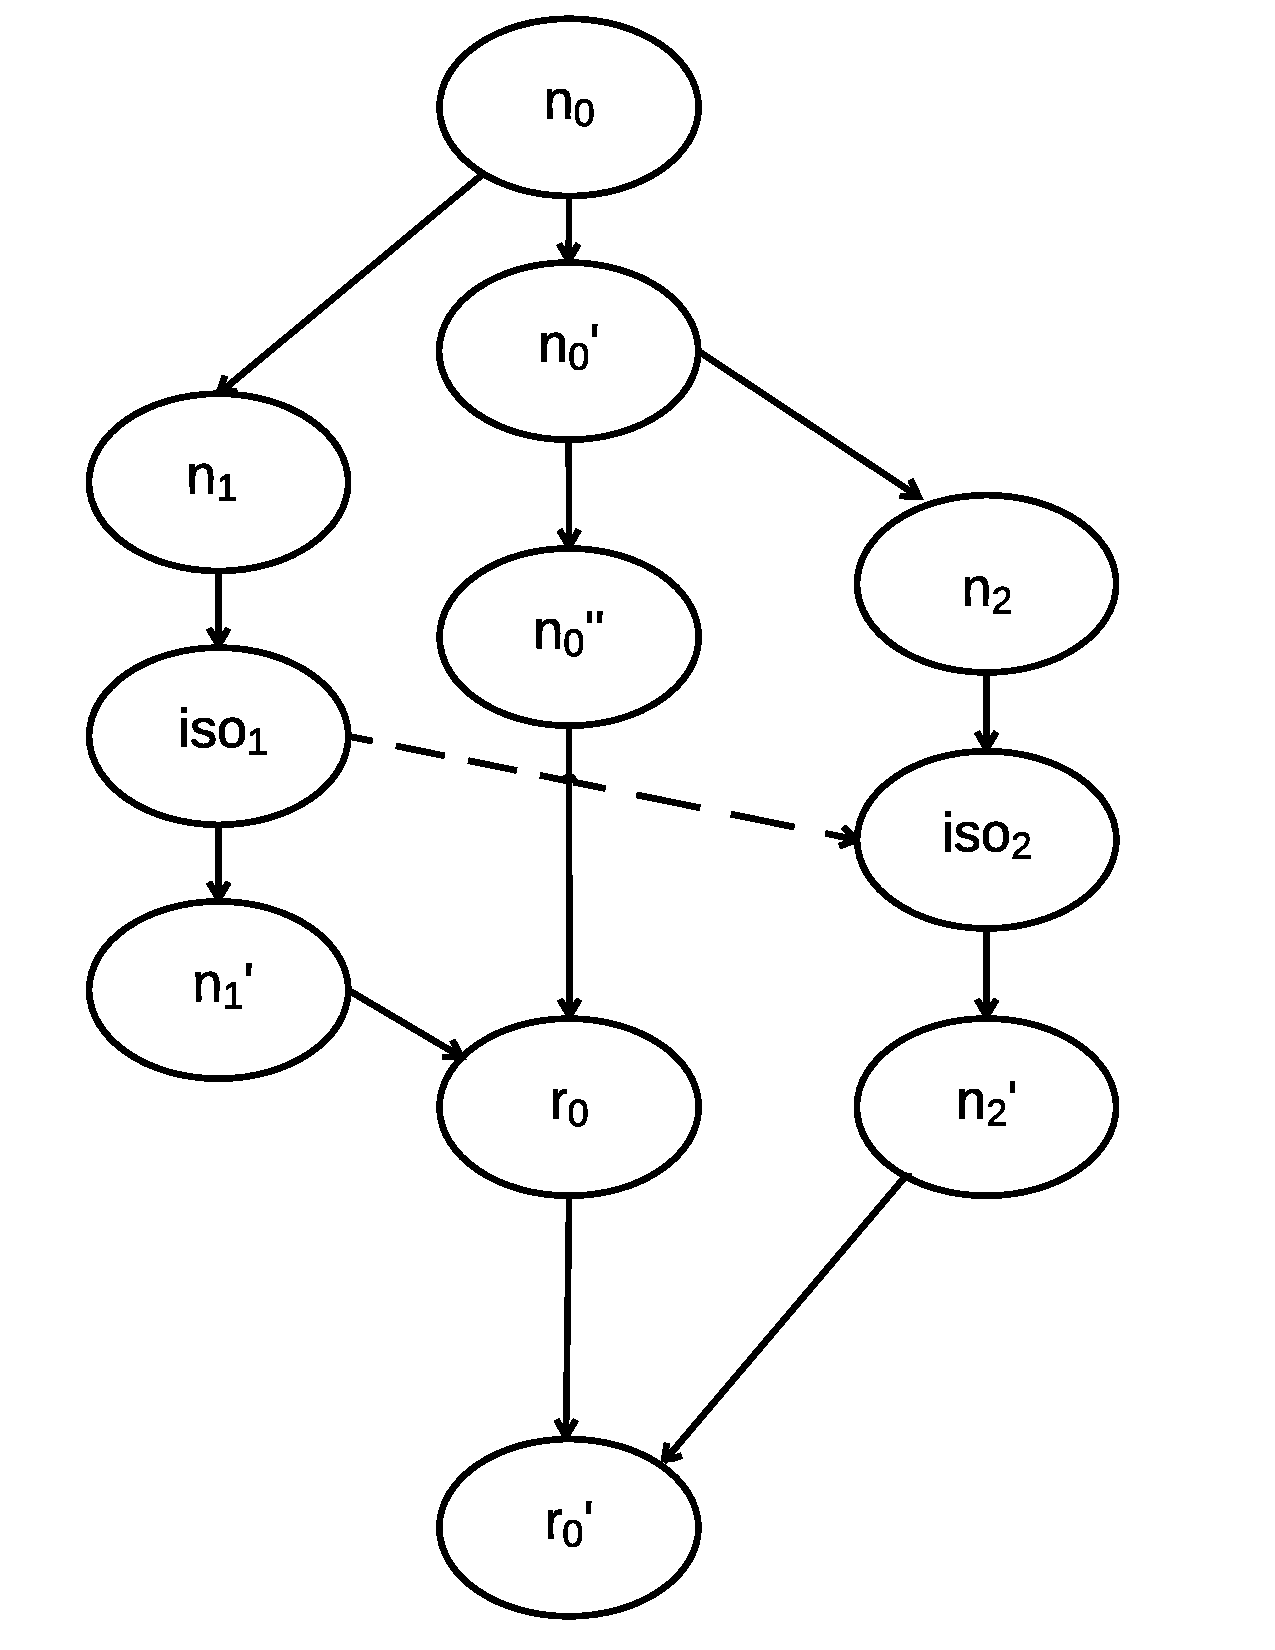
\includegraphics[scale=0.2]{../figs/Fig5-a.pdf}}
  \subfigure[p1 runs before p2.]{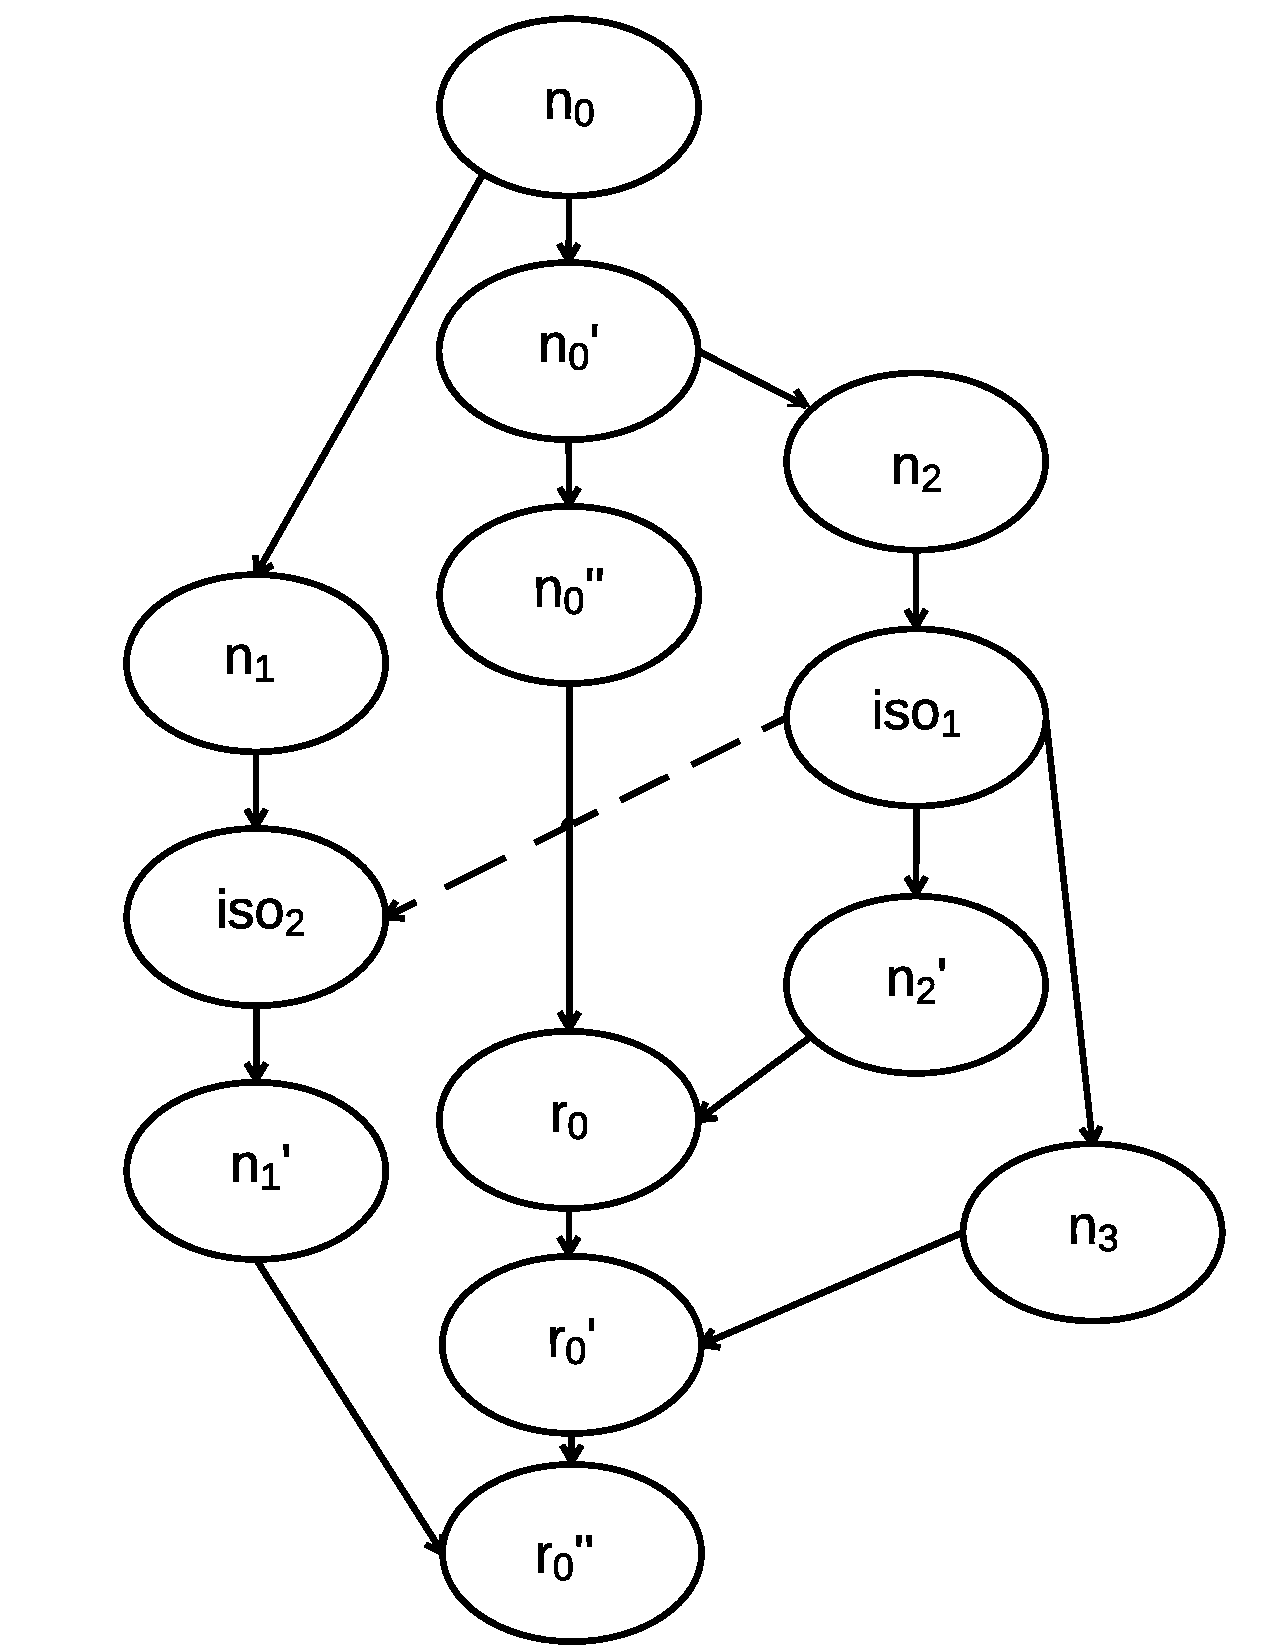
\includegraphics[scale=0.2]{../figs/Fig5-b.pdf}}
  \caption{Two possible computation graphs based on isolated schedules.}
  \vspace{-1em}
   \label{fig:cg-isolated}
\end{figure}

For the example in \figref{fig:hj-isolated}, two different computation graph structures can be formed based on the order of execution of isolated blocks. The computation graphs are shown in \figref{fig:cg-isolated}. The main task spawns two new tasks $t_1$ and $t_2$ both having isolated sections that run in mutual exclusion to each other. All the tasks have read/write access to region variable $r_1$. The isolated blocks are serialized by the runtime and based on the scheduler any task can execute its isolated section first. If the scheduler runs the isolated section of task $t_1$ first, the computation graph in \figref{fig:cg-isolated}(a) is formed. Task $t_1$ changes the values of shared variable $r_1$ to 2. Hence, when task $t_2$ executes its isolated section, the if-condition fails and an additional task is not spawned by $t_2$. If the scheduler runs task $t_2$ first, the computation graph of \figref{fig:cg-isolated}(b) is formed. In this schedule, task $t_2$ executes its isolated section first. Since the value of variable $r_1$ is 0, the if-condition is met and a new task is created by $t_2$.

\begin{theorem}
Algorithm \ref{algo:isolated} finds all unique computation graphs for structured parallel programs with isolated sections making it sound and complete with Algorithm \ref{algo:drd}.
\end{theorem}

\begin{proof}
%Theorem \ref{thm:strcutured-par-progs} 
\thmref{thm:strcutured-par-progs} 
states that Algorithm \ref{algo:drd} is sound and complete for structured parallel programs that do not contain isolated sections. If mutual exclusion is present, Algorithm \ref{algo:drd} does not remain sound since different computation graph structures can be formed for such programs. Algorithm \ref{algo:isolated} helps to enumerate all such computation graph structures. Therefore, the data race detection using Algorithm \ref{algo:drd} becomes sound and complete when it is used along with Algorithm \ref{algo:isolated} for structured parallel programs that have mutual exclusion.
\end{proof}


\chapter{Implementation and Results}
\section{Implementation and Results}
\label{sec:res}

The data race detection technique described in this paper has been implemented for Habanero Java. It uses the verification runtime specifically designed to test HJ programs \cite{anderson2014jpf}. This runtime makes use of JPF to schedule and run the programs. JPF is essentially a fully customizable Java virtual machine. JPF is modified by removing its default scheduling-factory that inserts choices on all thread actions and accesses to shared variables. Instead, a new scheduling factory based on Algorithm \ref{algo:isolated} is employed for scheduling. The computation graphs are stored in a directed acyclic graph \cite{jgrapht}. The computation graphs are exported in the dot file format for convenience and as a way to understand the structure of the program \cite{graphviz}.

The data-race detector is created by implementing the methods in the \textit{PropertyListenerAdapter} to create the computation graph. When the runtime passes an object of the type \textit{Task} to the \texttt{objectCreated} method, the \textsc{Post} rule is invoked that adds a new node to the computation graph. When the \textit{stop-finish} is executed, the \textsc{Await-next} rule is invoked that creates a node in the graph to synchronize the tasks in the finish block. The \texttt{executeInstruction} method is used to track memory locations that are accessed by various tasks by updating the node with the location accessed by the task during the execution of that instruction.

The results for this technique have been compared to two approaches implemented by JPF: \textit{Precise race detector} and \textit{Gradual permission regions} on benchmarks that cover a wide range of functionality in HJ. These two approaches are specifically chosen for comparison since the results generated by these approaches are sound for a given input just like the technique discussed in this paper. The results show a significant improvement in the time required for verification. 

The benchmarks used in this study make use of various HJ constructs for achieving task parallelism. They spawn a wide range of tasks with smaller programs having 3-15 tasks going all the way up to 525 tasks for larger programs. The experiments were run on a machine with an Intel Core i5 processor with 2.6GHz speed and 8GB of RAM.

\begin{table*}
\centering
\caption{Benchmarks of HJ programs: Computation graphs vs Permission Regions vs. PreciseRaceDetector}
\rowcolors{1}{light-gray}{white}
\label{tab:results}
\resizebox{\textwidth}{!}{
\begin{tabular}{|m{3.5cm}|c|c|c|c|c|c|c|c|c|c|c|}
\hiderowcolors
\hline
        &      &       & 
        \multicolumn{3}{c|}{\textbf{\textit{Computation graphs}}} & 
		 \multicolumn{3}{c|}{\textbf{\textit{Gradual permission regions}}} &
		\multicolumn{3}{c|}{\textbf{\textit{Precise race detector}}} \\ \hline
		
\textbf{Test ID }& \textbf{SLOC} & \textbf{Tasks} 
& \textbf{States}  & \textbf{Time}  & \textbf{Error Note }
& \textbf{States}  & \textbf{Time}  & \textbf{Error Note }
& \textbf{States}  & \textbf{Time}  & \textbf{Error Note }     \\ \hline

\showrowcolors

\textit{Primitive Array Race} & 39 & 3 
%& 5 & 00:00 & Race
& 5 & 00:00 & Race
& 5 & 00:00 & Race
& 220 & 00:00 & Race \\ \hline

\textit{Substring Search}  & 83 & 59 
%& 64 & 00:03 & Race
& 64 & 00:03 & Race
& 8 & 00:00 & Race 
& N/A & N/A & N/A \\ \hline

\textit{Reciprocal Array Sum} & 58 & 2
%& 12 & 0:00:16 & Race
& 4 & 00:08 & Race
& 32 & 00:06 & Race
& N/A & N/A & N/A \\ \hline

\textit{Primitive Array No Race} & 29 & 3 
%& 5 & 00:00 & No Race
& 5 & 00:00 & No Race
& 5 & 00:00 & No Race 
& 11,852 & 00:00 & No Race \\ \hline

\textit{Two Dim Arrays }& 30 & 11 
%& 15 & 00:01 & No Race
& 15 & 00:00 & No Race
& 15 & 00:00 & No Race 
& 597 & 00:00 & Race* \\ \hline

\textit{ForAll With Iterable} & 38 & 2
%& 9 & 00:00 & No Race
& 9 & 00:00 & No Race
& 9 & 00:00 & No Race 
& N/A & N/A & N/A \\ \hline

\textit{Integer Counter  Isolated} & 54 & 10
%& 24 & 00:01 & No Race
& 24 & 00:01 & No Race
& 1,013,102 & 05:53 & No Race 
& N/A & N/A & N/A \\ \hline

\textit{Pipeline With Futures} & 69 & 5
%& 34 & 0:00:00 & No Race
& 34 & 00:00 & No Race
& 34 & 00:00 & No Race 
& N/A & N/A & N/A \\ \hline

\textit{Binary Trees }& 80 & 525 
%& 632 & 0:00:05 & No Race
& 630 & 00:25 & No Race
& 632 & 00:03 & No Race 
& N/A & N/A & N/A \\ \hline

\textit{Prime Num Counter} & 51 & 25
%& 776 & 00:01 & No Race
& 776 & 00:01 & No Race
& 3,542,569 & 17:37 & No Race 
& N/A & N/A & N/A \\ \hline

\textit{Prime Num  Counter ForAll}  & 52 & 25
%& 30 & 0:00:02 & Race*
& 30 & 00:02 & No Race
& 18 & 00:01 & No Race
& N/A & N/A & N/A \\ \hline

\textit{Prime Num Counter ForAsync}  & 44 & 11 
%& 653 & 0:00:01 & No Race
& 653 & 00:01 & No Race
& 2,528,064 & 15:44 & No Race 
& N/A & N/A & N/A \\ \hline

\textit{Add}  & 67 & 3 
%& 11 & 0:00:01 & No Race 
& 11 & 00:01 & No Race 
& 62,374 & 00:33 & No Race
& 4930 & 00:03 & Race* \\ \hline

\textit{Scalar Multiply}  & 55 & 3 
%& 15 & 0:00:01 & No Race
& 15 & 00:01 & No Race
& 55,712 & 00:30 & No Race 
& 826 & 00:01 & Race* \\ \hline

\textit{Vector Add} & 50 & 3 
%& 5 & 0:00:01 & No Race
& 5 & 00:00 & No Race
& 17 & 00:00 & No Race 
& 46,394 & 00:19 & No Race \\ \hline

\textit{Clumped Access}  & 30 & 3 
%& 9 & 0:00:07 & No Race
& 5 & 00:03 & No Race
& 15 & 00:00 & No Race 
& N/A & N/A & N/A \\ \hline

\end{tabular}}
\vspace{-1em}
\end{table*}

\tableref{tab:results} presents the results of verification of the HJ benchmarks. The number of states explored by JPF and time required for verification by each method is compared. The tests are run for a maximum of an hour before they are terminated manually. If a test does not finish in the time bound or if it runs out of JVM memory, then it is marked as N/A in the table. The error note column shows the results of verification. The tests that produce erroneous results are marked with an asterisk ($\ast$). 

The \textit{Precise race detector} explores all potential executions of the program in a systematic way. Each execution is a sequence of transitions. Each transition takes the system from one state to another. Each transition consists of a sequence of byte-code instructions. JPF groups byte-code instructions such that an instruction that manipulates a shared variable is the first one of a transition. In every state that JPF visits, the \textit{precise race detector} checks all actions that can be performed next. If this collection of actions contains at least two conflicting accesses to a shared variable, then a data-race on the shared variable is reported. The \textit{precise race detector} inserts choices in the scheduler for all thread actions such as thread creation, synchronizations, locks etc. Therefore, it does not complete execution within the stipulated time or runs out of memory even on smaller programs because of the state space explosion. It also reports race for \textit{Two Dimensional Arrays}, \textit{Scalar multiply} and \textit{Vector Add} benchmarks where no data race actually exists in the program. This error is because in precise race detector, the access on an array object looks like a data race since it is not able to see the difference in the indexes.

\textit{Gradual permission regions} use program annotations to reduce the state space of the program \cite{mercer2015model}. Whenever a shared variable is accessed by multiple tasks in the program, the accesses have to be annotated to inform the data-race detector to create different schedules for these accesses. It is prone to human errors because of the need for manual annotation. If the program is annotated incorrectly, the results of data race detection analysis are no longer sound. \textit{gradual permission regions} works better than \textit{precise race detector}. Compared to \textit{computation graphs} in this paper though it falls behind quickly when there are several regions to annotate. A single execution is all that is needed for the \textit{computation graph analysis} while \textit{permission regions} have to enumerate an exponential number of schedules over the regions. The difference in performance is seen in the \textit{Add}, \textit{Scalar multiply} and \textit{Prime number counter} benchmarks. These benchmarks use shared variables that have to be enclosed within regions which results in a large state space for permission regions. The \textit{Prime number counter} benchmark also has isolated sections and therefore, the state space for \textit{computation graphs} is also large compared to other benchmarks.

We also evaluated our data race detector on some real world benchmarks. The \textit{Crypt-af} and \textit{Crypt-f} benchmarks are implementation of the IDEA encrytion algorithm and \textit{Series-af} and \textit{Series-f} are the Fourier coefficient analysis benchmarks adapted from the JGF suite \cite{bull2000benchmark} using \textbf{async-finish} and \textbf{future} constructs respectively. The \textit{strassen} benchmark is adapted from the  OpenMP version of the program in the Kastors suite \cite{virouleau:hal-01081974}. \tableref{tab:results1} shows the results of this evaluation.

\begin{table*}
\centering
\caption{Evaluation of Computation graphs on real world benchmarks}
\rowcolors{1}{light-gray}{white}
\label{tab:results1}
\begin{tabular}{|c|c|c|c|c|c|}
\hiderowcolors
\hline

\textbf{Test ID }& \textbf{SLOC} & \textbf{Tasks} 
& \textbf{States}  & \textbf{Time}  & \textbf{Error Note }\\ \hline

\showrowcolors

\textit{Crypt-af} & 1010 & 259
& 260 & 00:17 & No Race  \\ \hline

\textit{Crypt-f}  & 1145 & 387 
& 775 & 00:46 & No Race \\ \hline

\textit{Series-af} & 730 & 329
& 750 & 00:36 & No Race \\ \hline

\textit{Series-f} & 830 & 354 
& 630 & 00:51 & No Race\\ \hline

\textit{Strassen} & 560 & 3
& 7 & 00:57 & No Race \\ \hline

\end{tabular}
\vspace{-1em}
\end{table*}
\vspace{-2em}

\chapter{Related Work}
\section{Related Work} \label{sec:rel-work}
Data-race detection in \emph{unstructured thread parallelism}, where there is no defined protocol for creating and joining threads, or accessing shared memory, relies on static analysis to approximate parallelism and memory accesses \cite{schonberg1989fly,choi2001static,kahlon2009static,kulikov2010detecting,vechev2011automatic} and then improves precision with dynamic analysis \cite{lamport1978time,Godefroid,flanagan2009fasttrack,EraserUpgrade,dimitrov2014commutativity}. Other approaches reason about threads individually \cite{xu1997rely,flanagan2003thread,henzinger2003thread,malkis2007precise,gotsman2007thread}, rely on  assertions \cite{burnim2009asserting, burnim2010determin, hong2012testing, yu2012maple, terragni2015recontest, yu2014simrt, leon2015unfolding, kahkonen2015unfolding}, use low-overhead instrumentation \cite{nistor2010instantcheck}, or construct type proofs \cite{abadi2006types}. These approaches  make few assumptions about the parallelism for generality and typically have higher cost for analysis. 

\emph{Structured parallelism} constrains how threads are created and joined and how shared memory is accessed through programming models. For example, a locking protocol leads to static, dynamic, or hybrid lock-set analyses for data-race detection that are typically more efficient than approaches to unstructured parallelism \cite{savage1997eraser,engler2003racerx,locksets-msr,elmas2006goldilocks,naik2006effective,elmas2007goldilocks,voung2007relay,kahlon2010universal}. Locking protocols are not directly applicable to task-parallel programming models that also constrain parallelism but often without explicit locking. 

\begin{comment}
Different types of data race detection techniques have been developed. The static race detectors analyze the source code to detect races. The dynamic ones use information from the actual program executions. Another technique for data race detection is model checking. In this method, a model of the system being analyzed is created and whether this model meets the specifications is exhaustively checked.

Static data race detectors require program instrumentation by the users. They can reason about all possible program runs. The major drawback of these systems is that they produce a large number of false-positives. \cite{engler2003racerx,ESC,abadi2006types,naik2006effective,voung2007relay,choi2001static, vechev2011automatic}. 

Dynamic race detectors use use different techniques to detect data races at runtime. The lock-set based tools track the set of locks held by each task during execution. These sets are then used to determine conflicts over shared memory references \cite{savage1997eraser, EraserUpgrade, elmas2006goldilocks, elmas2007goldilocks}. 

Dimitrov et al. developed a dynamic commutativity race detector \cite{dimitrov2014commutativity}. It uses vector clocks along with a commutativity specification to generate a structural representation of parallel programs that is used to locate races. Dynamic race detectors based on hashing asserts if different runs of a parallel program with same input produce different outputs \cite{nistor2010instantcheck}.

Lamport defined the happens-before relation in parallel programs \cite{lamport1978time}. The happens-before relation defines a partial order among all the operations in all the threads of a parallel program. The happen-before relation has been used in various data race detection techniques \cite{kahlon2009static, kahlon2010universal, flanagan2009fasttrack, mellor1991fly, schonberg1989fly, miller1988mechanism}. This approach has also been applied to task parallel languages such as Cilk and X10 \cite{Feng97efficientdetection, Async-Finish-Race}. Two approaches based on the happens-before relation, discussed in the introduction, have been developed for HJ programs \cite{raman2012scalable, drdForFutures}. 

Model checking systematically explores the entire state space of the programs to detect concurrency issues \cite{kulikov2010detecting, vakkalanka2008implementing, Godefroid}. The major drawback of model checking is the explosion in the state space as the program size increases. This technique has been extended to verify various task parallel languages such as HJ, X10 and Chapel\cite{anderson2014jpf, gligoric2012x10x, zirkel2013automated}. As opposed to model checking, predictive analysis observes only a single program execution and generalizes the verification results to all possible schedules. This approach has been applied to detecting communication deadlocks in MPI programs \cite{forejt2014precise}.

Various methods have been developed to tackle the state explosion problem of model checking. Rely-guarantee reasoning verifies threads individually using assertions about other threads \cite{xu1997rely, popeea2012compositional}. Thread modular analysis relies on a similar technique. It verifies threads individually using an abstraction of steps that may be performed by other threads \cite{flanagan2003thread, malkis2007precise, henzinger2003thread, gotsman2007thread}.

Hybrid race detection systems have been developed that combine various techniques to overcome some of the limitations of these methods. Permission regions use static program instrumentation combined with dynamic analysis to detect races \cite{westbrook2012practical, westbrook2012permission}. Gradual permission regions use a similar program instrumentation along with model checking \cite{mercer2015model}. 

This work makes use of the happens-before relation for dynamic analysis of programs and use model checking to ensure all schedules are considered in programs with mutual exclusion. A lot of different techniques create model of programs from program executions and use the models for verification. SATCheck observes the program execution to build a concrete behavior model of program execution and using a SAT solver, it tries to find other interesting behaviors \cite{demsky2015satcheck}. Coverage driven testing uses program execution to create a model of the thread interleavings and shared memory accesses to identify unexplored thread interleavings \cite{hong2012testing, yu2012maple}. Regression testing tools for concurrent programs use changes in the program model to identify shared memory accesses that might be affected by the code changes and identifying thread interleavings that must be explored to expose regression bugs \cite{terragni2015recontest, yu2014simrt}. Dynamic symbolic execution is combined with unfolding of petri-nets to create minimal test-suites for testing multi-threaded programs \cite{leon2015unfolding, kahkonen2015unfolding}.
\end{comment}


\chapter{Conclusion and Future Work}
\section{Conclusion} \label{sec:conclusion}
This work presents a sound and complete technique for data race detection in task parallel programs using computation graphs.  The computation graph creation is presented with the formal semantics for task parallel languages. A scheduling algorithm to create all computation graph structures for programs containing mutual exclusion is also presented for use in model checking. The data race detection analysis is implemented for a Java implementation of the Habanero programming model using JPF and evaluated on a host of benchmarks. The results are compared to JPF's precise race detector and a gradual permission regions based extension. The results show that computation graph analysis reduces the time required for verification significantly relative to JPF's standards. 

\begin{comment}
This work can be extended in the following ways:
\begin{itemize}
\item The data race detector based on computation graphs explores just one control flow path that is taken by the program execution based on the input. The listener can be extended to explore other control flow paths by using Symbolic Execution.
\item The computation graphs can be created statically using program instrumentation and analyzed to gain performance improvements.
\end{itemize}
\end{comment}


\bibliographystyle{ieeetran}
\bibliography{../paper}

\end{document}